\documentclass[t]{beamer}

\usetheme{metropolis}

\usepackage{graphicx}
\usepackage{pgfplots}
\usepackage{pgfplotstable}
\usepackage{tikz}

\author{Esten H{\o}yland Leonardsen}
\date{31.08.22}
\title{Detecting individual-level deviations in brain morphology in MCI patients}

% TIKZ PACKAGES
\usetikzlibrary{arrows.meta}
\usetikzlibrary{calc}

% COLOUR
\definecolor{cb-pink}{HTML}{eeafcf}
\definecolor{cb-orange}{HTML}{e59145}
\definecolor{cb-light-brown}{HTML}{baa066}
\definecolor{cb-blue}{HTML}{3594d6}
\definecolor{cb-green}{HTML}{4dac93}
\definecolor{cb-gray}{HTML}{3a5c7d}
\definecolor{cb-light-purple}{HTML}{b45899}
\definecolor{cb-red-purple}{HTML}{c71555}
\definecolor{cb-brown}{HTML}{840000}
\definecolor{cb-blue-purple}{HTML}{662fa2}

\begin{document}

	\definecolor{outercolor}{RGB}{128, 128, 128}
	\newcommand{\nodesize}{11pt}
	\newcommand{\hsep}{28pt}
	\newcommand{\vsep}{14pt}

	\newcommand{\arrowwidth}{0.05cm}
	\newcommand{\innerarrow}{{Latex[length=0.1cm, width=0.15cm]}}
	\newcommand{\outerarrow}{{Latex[length=0.2cm, width=0.3cm]}}

	\titlepage
	\begin{frame}{Explainable AI}
		\vfill
		\centering
		\begin{tikzpicture}
			\newcommand{\mrilocation}[1]{($(0, -2.2)$)}
			\newcommand{\modellocation}[1]{($ (4.5, -2.2) + ####1 $)}

			\colorlet{predict-fill}{cb-blue}

			\node[inner sep=0pt, outer sep=0pt,draw=black] (input) at \mrilocation{(0, 0)} {
				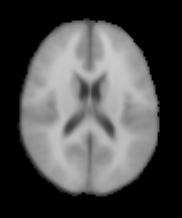
\includegraphics[width=1.2cm]{data/slice.png}
			};

			\node[circle, inner sep=0pt, fill=none, outer sep=0pt, line width=0pt, draw=none] (n00) at \modellocation{(-3 * \hsep, 0)} {};

			\node[circle, minimum size=\nodesize, inner sep=0pt, fill=predict-fill!85, outer sep=0pt, line width=0pt, draw=predict-fill!85] (n10) at \modellocation{(-2 * \hsep, 2 * \vsep)} {};
			\node[circle, minimum size=\nodesize, inner sep=0pt, fill=predict-fill, outer sep=0pt, line width=0pt, draw=predict-fill] (n11) at \modellocation{(-2 * \hsep, 1 * \vsep)} {};
			\node[circle, minimum size=\nodesize, inner sep=0pt, fill=predict-fill!75, outer sep=0pt, line width=0pt, draw=predict-fill!75] (n12) at \modellocation{(-2 * \hsep, 0)} {};
			\node[circle, minimum size=\nodesize, inner sep=0pt, fill=predict-fill!15, outer sep=0pt, line width=0pt, draw=predict-fill!15] (n13) at \modellocation{(-2 * \hsep, -1 * \vsep)} {};
			\node[circle, minimum size=\nodesize, inner sep=0pt, fill=predict-fill!50, outer sep=0pt, line width=0pt, draw=predict-fill!50] (n14) at \modellocation{(-2 * \hsep, -2 * \vsep)} {};

			\node[circle, minimum size=\nodesize, inner sep=0pt, fill=predict-fill!15, outer sep=0pt, line width=0pt, draw=predict-fill!15] (n20) at \modellocation{(-1 * \hsep, 1.5 * \vsep)} {};
			\node[circle, minimum size=\nodesize, inner sep=0pt, fill=predict-fill!65, outer sep=0pt, line width=0pt, draw=predict-fill!65] (n21) at \modellocation{(-1 * \hsep, 0.5 * \vsep)} {};
			\node[circle, minimum size=\nodesize, inner sep=0pt, fill=predict-fill!90, outer sep=0pt, line width=0pt, draw=predict-fill!90] (n22) at \modellocation{(-1 * \hsep, -0.5 * \vsep)} {};
			\node[circle, minimum size=\nodesize, inner sep=0pt, fill=predict-fill!40, outer sep=0pt, line width=0pt, draw=predict-fill!40] (n23) at \modellocation{(-1 * \hsep, -1.5 * \vsep)} {};

			\node[circle, minimum size=\nodesize, inner sep=0pt, fill=predict-fill!80, outer sep=0pt, line width=0pt, draw=predict-fill!80] (n30) at \modellocation{(0 * \hsep, 1.5 * \vsep)} {};
			\node[circle, minimum size=\nodesize, inner sep=0pt, fill=predict-fill!55, outer sep=0pt, line width=0pt, draw=predict-fill!55] (n31) at \modellocation{(0 * \hsep, 0.5 * \vsep)} {};
			\node[circle, minimum size=\nodesize, inner sep=0pt, fill=predict-fill!15, outer sep=0pt, line width=0pt, draw=predict-fill!15] (n32) at \modellocation{(0 * \hsep, -0.5 * \vsep)} {};
			\node[circle, minimum size=\nodesize, inner sep=0pt, fill=predict-fill!75, outer sep=0pt, line width=0pt, draw=predict-fill!75] (n33) at \modellocation{(0 * \hsep, -1.5 * \vsep)} {};

			\node[circle, minimum size=\nodesize, inner sep=0pt, fill=predict-fill, outer sep=0pt, line width=0pt, draw=predict-fill] (n40) at \modellocation{(1 * \hsep, 1*\vsep)} {};
			\node[circle, minimum size=\nodesize, inner sep=0pt, fill=predict-fill!20, outer sep=0pt, line width=0pt, draw=predict-fill!20] (n41) at \modellocation{(1 * \hsep, 0*\vsep)} {};
			\node[circle, minimum size=\nodesize, inner sep=0pt, fill=predict-fill!15, outer sep=0pt, line width=0pt, draw=predict-fill!15] (n42) at \modellocation{(1 * \hsep, -1*\vsep)} {};

			\node[circle, minimum size=\nodesize, inner sep=0pt, fill=predict-fill!75, outer sep=0pt, line width=0pt, draw=predict-fill!75] (n50) at \modellocation{(2 * \hsep, 1*\vsep)} {};
			\node[circle, minimum size=\nodesize, inner sep=0pt, fill=predict-fill!35, outer sep=0pt, line width=0pt, draw=predict-fill!35] (n51) at \modellocation{(2 * \hsep, 0*\vsep)} {};
			\node[circle, minimum size=\nodesize, inner sep=0pt, fill=predict-fill!65, outer sep=0pt, line width=0pt, draw=predict-fill!65] (n52) at \modellocation{(2 * \hsep, -1*\vsep)} {};

			\node[circle, minimum size=\nodesize, inner sep=0pt, fill=predict-fill!85, outer sep=0pt, line width=0pt, draw=predict-fill!85] (output) at \modellocation{(3 * \hsep, 0)} {};

			\node[] (diagnosis) at (9.3, -2.2) {\scriptsize{prediction}};

			\draw[
				color=predict-fill!85,
				-\innerarrow,
				line width=\arrowwidth
			] (n00) to [out=20,in=200] (n10) {};
			\draw[
				color=predict-fill,
				-\innerarrow,
				line width=\arrowwidth
			] (n00) to [out=10,in=190] (n11) {};
			\draw[
				color=predict-fill!75,
				-\innerarrow,
				line width=\arrowwidth
			] (n00) to [out=0,in=180] (n12) {};
			\draw[
				color=predict-fill!15,
				-\innerarrow,
				line width=\arrowwidth
			] (n00) to [out=-10,in=170] (n13) {};
			\draw[
				color=predict-fill!50,
				-\innerarrow,
				line width=\arrowwidth
			] (n00) to [out=-20,in=160] (n14) {};

			\draw[
				color=predict-fill!75,
				-\innerarrow,
				line width=\arrowwidth
			] (n10) to [out=-5,in=175] (n20) {};
			\draw[
				color=predict-fill!50,
				-\innerarrow,
				line width=\arrowwidth
			] (n10) to [out=-15,in=165] (n21) {};
			\draw[
				color=predict-fill!55,
				-\innerarrow,
				line width=\arrowwidth
			] (n10) to [out=-25,in=155] (n22) {};
			\draw[
				color=predict-fill!85,
				-\innerarrow,
				line width=\arrowwidth
			] (n10) to [out=-35,in=145] (n23) {};

			\draw[
				color=predict-fill!45,
				-\innerarrow,
				line width=\arrowwidth
			] (n11) to [out=5,in=185] (n20) {};
			\draw[
				color=predict-fill!50,
				-\innerarrow,
				line width=\arrowwidth
			] (n11) to [out=-5,in=175] (n21) {};
			\draw[
				color=predict-fill,
				-\innerarrow,
				line width=\arrowwidth
			] (n11) to [out=-15,in=165] (n22) {};
			\draw[
				color=predict-fill!15,
				-\innerarrow,
				line width=\arrowwidth
			] (n11) to [out=-25,in=155] (n23) {};

			\draw[
				color=predict-fill!35,
				-\innerarrow,
				line width=\arrowwidth
			] (n12) to [out=15,in=195] (n20) {};
			\draw[
				color=predict-fill!90,
				-\innerarrow,
				line width=\arrowwidth
			] (n12) to [out=5,in=185] (n21) {};
			\draw[
				color=predict-fill!80,
				-\innerarrow,
				line width=\arrowwidth
			] (n12) to [out=-5,in=175] (n22) {};
			\draw[
				color=predict-fill!20,
				-\innerarrow,
				line width=\arrowwidth
			] (n12) to [out=-15,in=165] (n23) {};

			\draw[
				color=predict-fill!55,
				-\innerarrow,
				line width=\arrowwidth
			] (n13) to [out=25,in=205] (n20) {};
			\draw[
				color=predict-fill!65,
				-\innerarrow,
				line width=\arrowwidth
			] (n13) to [out=15,in=195] (n21) {};
			\draw[
				color=predict-fill!35,
				-\innerarrow,
				line width=\arrowwidth
			] (n13) to [out=5,in=185] (n22) {};
			\draw[
				color=predict-fill!45,
				-\innerarrow,
				line width=\arrowwidth
			] (n13) to [out=-5,in=175] (n23) {};

			\draw[
				color=predict-fill!10,
				-\innerarrow,
				line width=\arrowwidth
			] (n14) to [out=35,in=215] (n20) {};
			\draw[
				color=predict-fill!90,
				-\innerarrow,
				line width=\arrowwidth
			] (n14) to [out=25,in=205] (n21) {};
			\draw[
				color=predict-fill!80,
				-\innerarrow,
				line width=\arrowwidth
			] (n14) to [out=15,in=195] (n22) {};
			\draw[
				color=predict-fill!35,
				-\innerarrow,
				line width=\arrowwidth
			] (n14) to [out=5,in=185] (n23) {};

			\draw[
				color=predict-fill!75,
				-\innerarrow,
				line width=\arrowwidth
			] (n20) to [out=0,in=180] (n30) {};
			\draw[
				color=predict-fill!50,
				-\innerarrow,
				line width=\arrowwidth
			] (n20) to [out=-10,in=170] (n31) {};
			\draw[
				color=predict-fill!85,
				-\innerarrow,
				line width=\arrowwidth
			] (n20) to [out=-20,in=160] (n32) {};
			\draw[
				color=predict-fill!45,
				-\innerarrow,
				line width=\arrowwidth
			] (n20) to [out=-30,in=150] (n33) {};

			\draw[
				color=predict-fill!20,
				-\innerarrow,
				line width=\arrowwidth
			] (n21) to [out=10,in=190] (n30) {};
			\draw[
				color=predict-fill!35,
				-\innerarrow,
				line width=\arrowwidth
			] (n21) to [out=0,in=180] (n31) {};
			\draw[
				color=predict-fill!15,
				-\innerarrow,
				line width=\arrowwidth
			] (n21) to [out=-10,in=170] (n32) {};
			\draw[
				color=predict-fill!90,
				-\innerarrow,
				line width=\arrowwidth
			] (n21) to [out=-20,in=160] (n33) {};

			\draw[
				color=predict-fill!65,
				-\innerarrow,
				line width=\arrowwidth
			] (n22) to [out=20,in=200] (n30) {};
			\draw[
				color=predict-fill!20,
				-\innerarrow,
				line width=\arrowwidth
			] (n22) to [out=10,in=190] (n31) {};
			\draw[
				color=predict-fill!30,
				-\innerarrow,
				line width=\arrowwidth
			] (n22) to [out=0,in=180] (n32) {};
			\draw[
				color=predict-fill!40,
				-\innerarrow,
				line width=\arrowwidth
			] (n22) to [out=-10,in=170] (n33) {};

			\draw[
				color=predict-fill,
				-\innerarrow,
				line width=\arrowwidth
			] (n23) to [out=30,in=210] (n30) {};
			\draw[
				color=predict-fill!15,
				-\innerarrow,
				line width=\arrowwidth
			] (n23) to [out=20,in=200] (n31) {};
			\draw[
				color=predict-fill!75,
				-\innerarrow,
				line width=\arrowwidth
			] (n23) to [out=10,in=190] (n32) {};
			\draw[
				color=predict-fill!35,
				-\innerarrow,
				line width=\arrowwidth
			] (n23) to [out=0,in=180] (n33) {};

			\draw[
				color=predict-fill!70,
				-\innerarrow,
				line width=\arrowwidth
			] (n30) to [out=-5,in=175] (n40) {};
			\draw[
				color=predict-fill!80,
				-\innerarrow,
				line width=\arrowwidth
			] (n30) to [out=-15,in=165] (n41) {};
			\draw[
				color=predict-fill!20,
				-\innerarrow,
				line width=\arrowwidth
			] (n30) to [out=-25,in=155] (n42) {};

			\draw[
				color=predict-fill!60,
				-\innerarrow,
				line width=\arrowwidth
			] (n31) to [out=5,in=185] (n40) {};
			\draw[
				color=predict-fill!95,
				-\innerarrow,
				line width=\arrowwidth
			] (n31) to [out=-5,in=175] (n41) {};
			\draw[
				color=predict-fill!35,
				-\innerarrow,
				line width=\arrowwidth
			] (n31) to [out=-15,in=165] (n42) {};

			\draw[
				color=predict-fill!75,
				-\innerarrow,
				line width=\arrowwidth
			] (n32) to [out=15,in=195] (n40) {};
			\draw[
				color=predict-fill!20,
				-\innerarrow,
				line width=\arrowwidth
			] (n32) to [out=5,in=185] (n41) {};
			\draw[
				color=predict-fill!15,
				-\innerarrow,
				line width=\arrowwidth
			] (n32) to [out=-5,in=175] (n42) {};

			\draw[
				color=predict-fill!40,
				-\innerarrow,
				line width=\arrowwidth
			] (n33) to [out=25,in=205] (n40) {};
			\draw[
				color=predict-fill!80,
				-\innerarrow,
				line width=\arrowwidth
			] (n33) to [out=15,in=195] (n41) {};
			\draw[
				color=predict-fill!50,
				-\innerarrow,
				line width=\arrowwidth
			] (n33) to [out=5,in=185] (n42) {};

			\draw[
				color=predict-fill!25,
				-\innerarrow,
				line width=\arrowwidth
			] (n40) to [out=0,in=180] (n50) {};
			\draw[
				color=predict-fill!50,
				-\innerarrow,
				line width=\arrowwidth
			] (n40) to [out=-10,in=170] (n51) {};
			\draw[
				color=predict-fill!45,
				-\innerarrow,
				line width=\arrowwidth
			] (n40) to [out=-20,in=160] (n52) {};

			\draw[
				color=predict-fill!90,
				-\innerarrow,
				line width=\arrowwidth
			] (n41) to [out=10,in=190] (n50) {};
			\draw[
				color=predict-fill!10,
				-\innerarrow,
				line width=\arrowwidth
			] (n41) to [out=0,in=180] (n51) {};
			\draw[
				color=predict-fill!75,
				-\innerarrow,
				line width=\arrowwidth
			] (n41) to [out=-10,in=170] (n52) {};

			\draw[
				color=predict-fill!60,
				-\innerarrow,
				line width=\arrowwidth
			] (n42) to [out=20,in=200] (n50) {};
			\draw[
				color=predict-fill!25,
				-\innerarrow,
				line width=\arrowwidth
			] (n42) to [out=10,in=190] (n51) {};
			\draw[
				color=predict-fill!15,
				-\innerarrow,
				line width=\arrowwidth
			] (n42) to [out=0,in=180] (n52) {};

			\draw[
				color=predict-fill!95,
				-\innerarrow,
				line width=\arrowwidth
			] (n50) to [out=-10,in=170] (output) {};
			\draw[
				color=predict-fill!25,
				-\innerarrow,
				line width=\arrowwidth
			] (n51) to [out=0,in=180] (output) {};
			\draw[
				color=predict-fill!50,
				-\innerarrow,
				line width=\arrowwidth
			] (n52) to [out=10,in=190] (output) {};

			\draw[black] (n00.center) --
						 ($ (n00) + (0, 2*\vsep+0.5*\nodesize+2pt) $) --
						 ($ (n00) + (6*\hsep+0.5*\nodesize+2pt, 2*\vsep+0.5*\nodesize+2pt) $) --
						 ($ (n00) + (6*\hsep+0.5*\nodesize+2pt, -2*\vsep-0.5*\nodesize-2pt) $) --
						 ($ (n00) + (0, -2*\vsep-0.5*\nodesize-2pt) $) -- (n00.center);

			\node[text depth=0] at ($ (n30) + (0, \vsep+0.5*\nodesize) $) {\footnotesize{Prediction model}};

			\draw[
				color=outercolor,
				-\outerarrow,
				line width=0.1cm
			] (input) to [out=0,in=180] (n00) {};
			\draw[
				color=outercolor,
				-\outerarrow,
				line width=0.1cm
			] (output) to [out=0,in=180] (diagnosis) {};
		\end{tikzpicture}
		\vfill
	\end{frame}

	\begin{frame}{Explainable AI}
		\vfill
		\centering
		\begin{tikzpicture}
			\newcommand{\mrilocation}[1]{($(0, -2.2)$)}
			\newcommand{\lrplocation}[1]{($ (4.5, -2.2) + ####1 $)}

			\node[inner sep=0pt, outer sep=0pt, minimum width=1.2cm] (input) at \mrilocation{(0, 0)} {};

			\node[circle, inner sep=0pt, fill=none, outer sep=0pt, line width=0pt, draw=none] (n00) at \lrplocation{(-3 * \hsep, 0)} {};

			\node[circle, minimum size=\nodesize, inner sep=0pt, fill={rgb:black,5;orange,1}, outer sep=0pt, line width=0pt, draw={rgb:black,5;orange,1}] (n10) at \lrplocation{(-2 * \hsep, 2 * \vsep)} {};
			\node[circle, minimum size=\nodesize, inner sep=0pt, fill={rgb:black,3;red,1}, outer sep=0pt, line width=0pt, draw={rgb:black,3;red,1}] (n11) at \lrplocation{(-2 * \hsep, 1 * \vsep)} {};
			\node[circle, minimum size=\nodesize, inner sep=0pt, fill=yellow, outer sep=0pt, line width=0pt, draw=yellow] (n12) at \lrplocation{(-2 * \hsep, 0)} {};
			\node[circle, minimum size=\nodesize, inner sep=0pt, fill=black, outer sep=0pt, line width=0pt, draw=black] (n13) at \lrplocation{(-2 * \hsep, -1 * \vsep)} {};
			\node[circle, minimum size=\nodesize, inner sep=0pt, fill=red, outer sep=0pt, line width=0pt, draw=red] (n14) at \lrplocation{(-2 * \hsep, -2 * \vsep)} {};

			\node[circle, minimum size=\nodesize, inner sep=0pt, fill={rgb:black,5;white,2;orange,1}, outer sep=0pt, line width=0pt, draw={rgb:black,5;white,2;orange,1}] (n20) at \lrplocation{(-1 * \hsep, 1.5 * \vsep)} {};
			\node[circle, minimum size=\nodesize, inner sep=0pt, fill={rgb:red,10;yellow,6}, outer sep=0pt, line width=0pt, draw={rgb:red,10;yellow,4}] (n21) at \lrplocation{(-1 * \hsep, 0.5 * \vsep)} {};
			\node[circle, minimum size=\nodesize, inner sep=0pt, fill={rgb:red,10;yellow,1}, outer sep=0pt, line width=0pt, draw={rgb:red,10;yellow,1}] (n22) at \lrplocation{(-1 * \hsep, -0.5 * \vsep)} {};
			\node[circle, minimum size=\nodesize, inner sep=0pt, fill={rgb:black,10;red,2}, outer sep=0pt, line width=0pt, draw={rgb:black,10;red,2}] (n23) at \lrplocation{(-1 * \hsep, -1.5 * \vsep)} {};

			\node[circle, minimum size=\nodesize, inner sep=0pt, fill={rgb:red,3;orange,2}, outer sep=0pt, line width=0pt, draw={rgb:red,3;orange,1}] (n30) at \lrplocation{(0 * \hsep, 1.5 * \vsep)} {};
			\node[circle, minimum size=\nodesize, inner sep=0pt, fill={rgb:yellow,3;orange,1}, outer sep=0pt, line width=0pt, draw={rgb:yellow,3;orange,1}] (n31) at \lrplocation{(0 * \hsep, 0.5 * \vsep)} {};
			\node[circle, minimum size=\nodesize, inner sep=0pt, fill={rgb:black,10;white,5;red,1}, outer sep=0pt, line width=0pt, draw={rgb:black,10;white,5;red,1}] (n32) at \lrplocation{(0 * \hsep, -0.5 * \vsep)} {};
			\node[circle, minimum size=\nodesize, inner sep=0pt, fill={rgb:gray,5;red,1}, outer sep=0pt, line width=0pt, draw={rgb:gray,5;red,1}] (n33) at \lrplocation{(0 * \hsep, -1.5 * \vsep)} {};

			\node[circle, minimum size=\nodesize, inner sep=0pt, fill={rgb:yellow,10;orange,1}, outer sep=0pt, line width=0pt, draw={rgb:yellow,10;orange,1}] (n40) at \lrplocation{(1 * \hsep, 1*\vsep)} {};
			\node[circle, minimum size=\nodesize, inner sep=0pt, fill={rgb:red,1}, outer sep=0pt, line width=0pt, draw={rgb:red,1}] (n41) at \lrplocation{(1 * \hsep, 0*\vsep)} {};
			\node[circle, minimum size=\nodesize, inner sep=0pt, fill={rgb:black,10;white,15;red,2}, outer sep=0pt, line width=0pt, draw={rgb:black,10;white,15;red,2}] (n42) at \lrplocation{(1 * \hsep, -1*\vsep)} {};

			\node[circle, minimum size=\nodesize, inner sep=0pt, fill={rgb:red,5;black,1;yellow,2}, outer sep=0pt, line width=0pt, draw={rgb:red,5;black,1;yellow,2}] (n50) at \lrplocation{(2 * \hsep, 1*\vsep)} {};
			\node[circle, minimum size=\nodesize, inner sep=0pt, fill={rgb:gray,5;red,1}, outer sep=0pt, line width=0pt, draw={rgb:gray,5;red,1}] (n51) at \lrplocation{(2 * \hsep, 0*\vsep)} {};
			\node[circle, minimum size=\nodesize, inner sep=0pt, fill={rgb:yellow,5;orange,1}, outer sep=0pt, line width=0pt, draw={rgb:yellow,5;orange,1}] (n52) at \lrplocation{(2 * \hsep, -1*\vsep)} {};

			\node[circle, minimum size=\nodesize, inner sep=0pt, fill={rgb:orange,7;yellow,4;black,1}, outer sep=0pt, line width=0pt, draw={rgb:orange,7;yellow,4;black,1}] (n60) at \lrplocation{(3 * \hsep, 0)} {};

			\draw[
				color={rgb:black,5;orange,1},
				\innerarrow-,
				line width=\arrowwidth
			] (n00) to [out=20,in=200] (n10) {};
			\draw[
				color={rgb:black,3;red,1},
				\innerarrow-,
				line width=\arrowwidth
			] (n00) to [out=10,in=190] (n11) {};
			\draw[
				color=yellow,
				\innerarrow-,
				line width=\arrowwidth
			] (n00) to [out=0,in=180] (n12) {};
			\draw[
				color=black,
				\innerarrow-,
				line width=\arrowwidth
			] (n00) to [out=-10,in=170] (n13) {};
			\draw[
				color=red,
				\innerarrow-,
				line width=\arrowwidth
			] (n00) to [out=-20,in=160] (n14) {};

			\draw[
				color={rgb:black,5;white,1;orange,1},
				\innerarrow-,
				line width=\arrowwidth
			] (n10) to [out=-5,in=175] (n20) {};
			\draw[
				color={rgb:black,3;orange,1},
				\innerarrow-,
				line width=\arrowwidth
			] (n10) to [out=-15,in=165] (n21) {};
			\draw[
				color={rgb:black,4;red,2;yellow,1},
				\innerarrow-,
				line width=\arrowwidth
			] (n10) to [out=-25,in=155] (n22) {};
			\draw[
				color={rgb:black,3;red,1},
				\innerarrow-,
				line width=\arrowwidth
			] (n10) to [out=-35,in=145] (n23) {};

			\draw[
				color={rgb:black,10;orange,2},
				\innerarrow-,
				line width=\arrowwidth
			] (n11) to [out=5,in=185] (n20) {};
			\draw[
				color={rgb:black,3;orange,1},
				\innerarrow-,
				line width=\arrowwidth
			] (n11) to [out=-5,in=175] (n21) {};
			\draw[
				color={rgb:black,3;red,1},
				\innerarrow-,
				line width=\arrowwidth
			] (n11) to [out=-15,in=165] (n22) {};
			\draw[
				color={rgb:black,10;red,1},
				\innerarrow-,
				line width=\arrowwidth
			] (n11) to [out=-25,in=155] (n23) {};

			\draw[
				color={rgb:black,5;orange,3},
				\innerarrow-,
				line width=\arrowwidth
			] (n12) to [out=15,in=195] (n20) {};
			\draw[
				color={rgb:red,3;yellow,5},
				\innerarrow-,
				line width=\arrowwidth
			] (n12) to [out=5,in=185] (n21) {};
			\draw[
				color={rgb:red,5;yellow,3},
				\innerarrow-,
				line width=\arrowwidth
			] (n12) to [out=-5,in=175] (n22) {};
			\draw[
				color={rgb:black,5;orange,2},
				\innerarrow-,
				line width=\arrowwidth
			] (n12) to [out=-15,in=165] (n23) {};

			\draw[
				color={rgb:black,5;red,1},
				\innerarrow-,
				line width=\arrowwidth
			] (n13) to [out=25,in=205] (n20) {};
			\draw[
				color={rgb:black,5;orange,2},
				\innerarrow-,
				line width=\arrowwidth
			] (n13) to [out=15,in=195] (n21) {};
			\draw[
				color={rgb:black,5;red,3},
				\innerarrow-,
				line width=\arrowwidth
			] (n13) to [out=5,in=185] (n22) {};
			\draw[
				color=black,
				\innerarrow-,
				line width=\arrowwidth
			] (n13) to [out=-5,in=175] (n23) {};

			\draw[
				color={rgb:black,5;orange,2},
				\innerarrow-,
				line width=\arrowwidth
			] (n14) to [out=35,in=215] (n20) {};
			\draw[
				color={rgb:red,3;orange,1},
				\innerarrow-,
				line width=\arrowwidth
			] (n14) to [out=25,in=205] (n21) {};
			\draw[
				color={rgb:red,5;yellow,2},
				\innerarrow-,
				line width=\arrowwidth
			] (n14) to [out=15,in=195] (n22) {};
			\draw[
				color={rgb:black,5;red,3},
				\innerarrow-,
				line width=\arrowwidth
			] (n14) to [out=5,in=185] (n23) {};

			\draw[
				color={rgb:black,1;red,1},
				\innerarrow-,
				line width=\arrowwidth
			] (n20) to [out=0,in=180] (n30) {};
			\draw[
				color={rgb:black,3;orange,1},
				\innerarrow-,
				line width=\arrowwidth
			] (n20) to [out=-10,in=170] (n31) {};
			\draw[
				color={rgb:black,10;red,1},
				\innerarrow-,
				line width=\arrowwidth
			] (n20) to [out=-20,in=160] (n32) {};
			\draw[
				color={rgb:black,5;red,1},
				\innerarrow-,
				line width=\arrowwidth
			] (n20) to [out=-30,in=150] (n33) {};

			\draw[
				color={rgb:orange,5;red,2},
				\innerarrow-,
				line width=\arrowwidth
			] (n21) to [out=10,in=190] (n30) {};
			\draw[
				color={rgb:yellow,10;orange,4},
				\innerarrow-,
				line width=\arrowwidth
			] (n21) to [out=0,in=180] (n31) {};
			\draw[
				color={rgb:black,2;red,1},
				\innerarrow-,
				line width=\arrowwidth
			] (n21) to [out=-10,in=170] (n32) {};
			\draw[
				color={rgb:black,1;orange,2;red,1},
				\innerarrow-,
				line width=\arrowwidth
			] (n21) to [out=-20,in=160] (n33) {};

			\draw[
				color={rgb:red,2;orange,1},
				\innerarrow-,
				line width=\arrowwidth
			] (n22) to [out=20,in=200] (n30) {};
			\draw[
				color={rgb:yellow,2;orange,1},
				\innerarrow-,
				line width=\arrowwidth
			] (n22) to [out=10,in=190] (n31) {};
			\draw[
				color={rgb:black,2;red,2},
				\innerarrow-,
				line width=\arrowwidth
			] (n22) to [out=0,in=180] (n32) {};
			\draw[
				color={rgb:black,2;orange,1},
				\innerarrow-,
				line width=\arrowwidth
			] (n22) to [out=-10,in=170] (n33) {};

			\draw[
				color={rgb:black,4;red,2},
				\innerarrow-,
				line width=\arrowwidth
			] (n23) to [out=30,in=210] (n30) {};
			\draw[
				color={rgb:orange,2;black,1},
				\innerarrow-,
				line width=\arrowwidth
			] (n23) to [out=20,in=200] (n31) {};
			\draw[
				color={rgb:black,5;orange,1},
				\innerarrow-,
				line width=\arrowwidth
			] (n23) to [out=10,in=190] (n32) {};
			\draw[
				color={rgb:black,5;red,2},
				\innerarrow-,
				line width=\arrowwidth
			] (n23) to [out=0,in=180] (n33) {};

			\draw[
				color={rgb:orange,3;red,1},
				\innerarrow-,
				line width=\arrowwidth
			] (n30) to [out=-5,in=175] (n40) {};
			\draw[
				color={rgb:gray,1;orange,1;red,2},
				\innerarrow-,
				line width=\arrowwidth
			] (n30) to [out=-15,in=165] (n41) {};
			\draw[
				color={rgb:orange,2;black,2;white,1},
				\innerarrow-,
				line width=\arrowwidth
			] (n30) to [out=-25,in=155] (n42) {};

			\draw[
				color={rgb:yellow,5;orange,1},
				\innerarrow-,
				line width=\arrowwidth
			] (n31) to [out=5,in=185] (n40) {};
			\draw[
				color={rgb:red,3;orange,1},
				\innerarrow-,
				line width=\arrowwidth
			] (n31) to [out=-5,in=175] (n41) {};
			\draw[
				color={rgb:gray,1;red,2},
				\innerarrow-,
				line width=\arrowwidth
			] (n31) to [out=-15,in=165] (n42) {};

			\draw[
				color={rgb:gray,3;orange,1},
				\innerarrow-,
				line width=\arrowwidth
			] (n32) to [out=15,in=195] (n40) {};
			\draw[
				color={rgb:gray,1;red,1},
				\innerarrow-,
				line width=\arrowwidth
			] (n32) to [out=5,in=185] (n41) {};
			\draw[
				color={rgb:gray,1},
				\innerarrow-,
				line width=\arrowwidth
			] (n32) to [out=-5,in=175] (n42) {};

			\draw[
				color={rgb:gray,2;orange,3},
				\innerarrow-,
				line width=\arrowwidth
			] (n33) to [out=25,in=205] (n40) {};
			\draw[
				color={rgb:gray,1;orange,1},
				\innerarrow-,
				line width=\arrowwidth
			] (n33) to [out=15,in=195] (n41) {};
			\draw[
				color={rgb:gray,3;red,1},
				\innerarrow-,
				line width=\arrowwidth
			] (n33) to [out=5,in=185] (n42) {};

			\draw[
				color={rgb:red,3;yellow,1},
				\innerarrow-,
				line width=\arrowwidth
			] (n40) to [out=0,in=180] (n50) {};
			\draw[
				color={rgb:gray,2;orange,1},
				\innerarrow-,
				line width=\arrowwidth
			] (n40) to [out=-10,in=170] (n51) {};
			\draw[
				color={rgb:yellow,10;orange,1},
				\innerarrow-,
				line width=\arrowwidth
			] (n40) to [out=-20,in=160] (n52) {};

			\draw[
				color={rgb:red,5;black,1;yellow,2},
				\innerarrow-,
				line width=\arrowwidth
			] (n41) to [out=10,in=190] (n50) {};
			\draw[
				color={rgb:gray,7;orange,3},
				\innerarrow-,
				line width=\arrowwidth
			] (n41) to [out=0,in=180] (n51) {};
			\draw[
				color={rgb:yellow,1;orange,2},
				\innerarrow-,
				line width=\arrowwidth
			] (n41) to [out=-10,in=170] (n52) {};

			\draw[
				color={rgb:gray,7;orange,2},
				\innerarrow-,
				line width=\arrowwidth
			] (n42) to [out=20,in=200] (n50) {};
			\draw[
				color={rgb:gray,5;red,1},
				\innerarrow-,
				line width=\arrowwidth
			] (n42) to [out=10,in=190] (n51) {};
			\draw[
				color={rgb:gray,5;red,1;black,2},
				\innerarrow-,
				line width=\arrowwidth
			] (n42) to [out=0,in=180] (n52) {};

			\draw[
				color={rgb:red,5;black,1;yellow,2},
				\innerarrow-,
				line width=\arrowwidth
			] (n50) to [out=-10,in=170] (n60) {};
			\draw[
				color={rgb:gray,5;red,1},
				\innerarrow-,
				line width=\arrowwidth
			] (n51) to [out=0,in=180] (n60) {};
			\draw[
				color={rgb:yellow,5;orange,1},
				\innerarrow-,
				line width=\arrowwidth
			] (n52) to [out=10,in=190] (n60) {};

			\draw[black] (n00.center) --
						($ (n00) + (0, 2*\vsep+0.5*\nodesize+2pt) $) --
						($ (n00) + (6*\hsep+0.5*\nodesize+2pt, 2*\vsep+0.5*\nodesize+2pt) $) --
						($ (n00) + (6*\hsep+0.5*\nodesize+2pt, -2*\vsep-0.5*\nodesize-2pt) $) --
						($ (n00) + (0, -2*\vsep-0.5*\nodesize-2pt) $) -- (n00.center);

			\node[text depth=0] at ($ (n30) + (0, \vsep+0.5*\nodesize) $) {\footnotesize{Layerwise Relevance Propagation}};

			\node[] (diagnosis) at (9.3, -2.2) {\scriptsize{prediction}};


			\draw[
				color=outercolor,
				\outerarrow-,
				line width=0.1cm
			] (output) to [out=0,in=180] (diagnosis) {};

		\end{tikzpicture}
		\vfill
	\end{frame}

	\begin{frame}{Explainable AI}
		\vfill
		\centering
		\begin{tikzpicture}
			\newcommand{\mrilocation}[1]{($(0, -2.2)$)}
			\newcommand{\lrplocation}[1]{($ (4.5, -2.2) + ####1 $)}

			\node[inner sep=0pt, outer sep=0pt, minimum width=1.2cm] (input) at \mrilocation{(0, 0)} {
				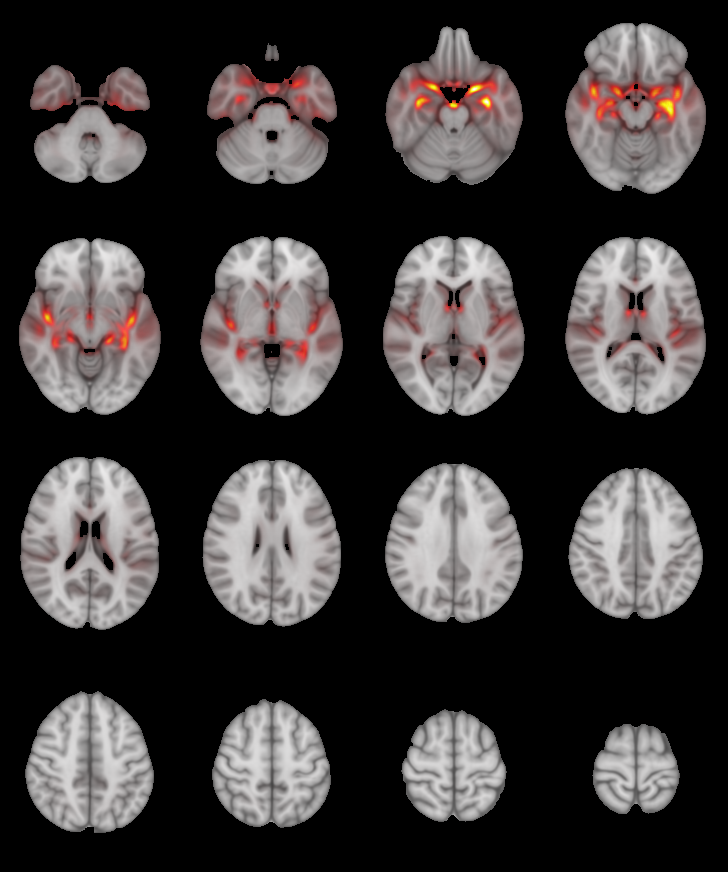
\includegraphics[
					width=1.2cm,
					clip=true,
					trim = 192mm 232mm 0mm 0mm
				]{data/dementia_average.png}
			};

			\node[circle, inner sep=0pt, fill=none, outer sep=0pt, line width=0pt, draw=none] (n00) at \lrplocation{(-3 * \hsep, 0)} {};

			\node[circle, minimum size=\nodesize, inner sep=0pt, fill={rgb:black,5;orange,1}, outer sep=0pt, line width=0pt, draw={rgb:black,5;orange,1}] (n10) at \lrplocation{(-2 * \hsep, 2 * \vsep)} {};
			\node[circle, minimum size=\nodesize, inner sep=0pt, fill={rgb:black,3;red,1}, outer sep=0pt, line width=0pt, draw={rgb:black,3;red,1}] (n11) at \lrplocation{(-2 * \hsep, 1 * \vsep)} {};
			\node[circle, minimum size=\nodesize, inner sep=0pt, fill=yellow, outer sep=0pt, line width=0pt, draw=yellow] (n12) at \lrplocation{(-2 * \hsep, 0)} {};
			\node[circle, minimum size=\nodesize, inner sep=0pt, fill=black, outer sep=0pt, line width=0pt, draw=black] (n13) at \lrplocation{(-2 * \hsep, -1 * \vsep)} {};
			\node[circle, minimum size=\nodesize, inner sep=0pt, fill=red, outer sep=0pt, line width=0pt, draw=red] (n14) at \lrplocation{(-2 * \hsep, -2 * \vsep)} {};

			\node[circle, minimum size=\nodesize, inner sep=0pt, fill={rgb:black,5;white,2;orange,1}, outer sep=0pt, line width=0pt, draw={rgb:black,5;white,2;orange,1}] (n20) at \lrplocation{(-1 * \hsep, 1.5 * \vsep)} {};
			\node[circle, minimum size=\nodesize, inner sep=0pt, fill={rgb:red,10;yellow,6}, outer sep=0pt, line width=0pt, draw={rgb:red,10;yellow,4}] (n21) at \lrplocation{(-1 * \hsep, 0.5 * \vsep)} {};
			\node[circle, minimum size=\nodesize, inner sep=0pt, fill={rgb:red,10;yellow,1}, outer sep=0pt, line width=0pt, draw={rgb:red,10;yellow,1}] (n22) at \lrplocation{(-1 * \hsep, -0.5 * \vsep)} {};
			\node[circle, minimum size=\nodesize, inner sep=0pt, fill={rgb:black,10;red,2}, outer sep=0pt, line width=0pt, draw={rgb:black,10;red,2}] (n23) at \lrplocation{(-1 * \hsep, -1.5 * \vsep)} {};

			\node[circle, minimum size=\nodesize, inner sep=0pt, fill={rgb:red,3;orange,2}, outer sep=0pt, line width=0pt, draw={rgb:red,3;orange,1}] (n30) at \lrplocation{(0 * \hsep, 1.5 * \vsep)} {};
			\node[circle, minimum size=\nodesize, inner sep=0pt, fill={rgb:yellow,3;orange,1}, outer sep=0pt, line width=0pt, draw={rgb:yellow,3;orange,1}] (n31) at \lrplocation{(0 * \hsep, 0.5 * \vsep)} {};
			\node[circle, minimum size=\nodesize, inner sep=0pt, fill={rgb:black,10;white,5;red,1}, outer sep=0pt, line width=0pt, draw={rgb:black,10;white,5;red,1}] (n32) at \lrplocation{(0 * \hsep, -0.5 * \vsep)} {};
			\node[circle, minimum size=\nodesize, inner sep=0pt, fill={rgb:gray,5;red,1}, outer sep=0pt, line width=0pt, draw={rgb:gray,5;red,1}] (n33) at \lrplocation{(0 * \hsep, -1.5 * \vsep)} {};

			\node[circle, minimum size=\nodesize, inner sep=0pt, fill={rgb:yellow,10;orange,1}, outer sep=0pt, line width=0pt, draw={rgb:yellow,10;orange,1}] (n40) at \lrplocation{(1 * \hsep, 1*\vsep)} {};
			\node[circle, minimum size=\nodesize, inner sep=0pt, fill={rgb:red,1}, outer sep=0pt, line width=0pt, draw={rgb:red,1}] (n41) at \lrplocation{(1 * \hsep, 0*\vsep)} {};
			\node[circle, minimum size=\nodesize, inner sep=0pt, fill={rgb:black,10;white,15;red,2}, outer sep=0pt, line width=0pt, draw={rgb:black,10;white,15;red,2}] (n42) at \lrplocation{(1 * \hsep, -1*\vsep)} {};

			\node[circle, minimum size=\nodesize, inner sep=0pt, fill={rgb:red,5;black,1;yellow,2}, outer sep=0pt, line width=0pt, draw={rgb:red,5;black,1;yellow,2}] (n50) at \lrplocation{(2 * \hsep, 1*\vsep)} {};
			\node[circle, minimum size=\nodesize, inner sep=0pt, fill={rgb:gray,5;red,1}, outer sep=0pt, line width=0pt, draw={rgb:gray,5;red,1}] (n51) at \lrplocation{(2 * \hsep, 0*\vsep)} {};
			\node[circle, minimum size=\nodesize, inner sep=0pt, fill={rgb:yellow,5;orange,1}, outer sep=0pt, line width=0pt, draw={rgb:yellow,5;orange,1}] (n52) at \lrplocation{(2 * \hsep, -1*\vsep)} {};

			\node[circle, minimum size=\nodesize, inner sep=0pt, fill={rgb:orange,7;yellow,4;black,1}, outer sep=0pt, line width=0pt, draw={rgb:orange,7;yellow,4;black,1}] (n60) at \lrplocation{(3 * \hsep, 0)} {};

			\draw[
				color={rgb:black,5;orange,1},
				\innerarrow-,
				line width=\arrowwidth
			] (n00) to [out=20,in=200] (n10) {};
			\draw[
				color={rgb:black,3;red,1},
				\innerarrow-,
				line width=\arrowwidth
			] (n00) to [out=10,in=190] (n11) {};
			\draw[
				color=yellow,
				\innerarrow-,
				line width=\arrowwidth
			] (n00) to [out=0,in=180] (n12) {};
			\draw[
				color=black,
				\innerarrow-,
				line width=\arrowwidth
			] (n00) to [out=-10,in=170] (n13) {};
			\draw[
				color=red,
				\innerarrow-,
				line width=\arrowwidth
			] (n00) to [out=-20,in=160] (n14) {};

			\draw[
				color={rgb:black,5;white,1;orange,1},
				\innerarrow-,
				line width=\arrowwidth
			] (n10) to [out=-5,in=175] (n20) {};
			\draw[
				color={rgb:black,3;orange,1},
				\innerarrow-,
				line width=\arrowwidth
			] (n10) to [out=-15,in=165] (n21) {};
			\draw[
				color={rgb:black,4;red,2;yellow,1},
				\innerarrow-,
				line width=\arrowwidth
			] (n10) to [out=-25,in=155] (n22) {};
			\draw[
				color={rgb:black,3;red,1},
				\innerarrow-,
				line width=\arrowwidth
			] (n10) to [out=-35,in=145] (n23) {};

			\draw[
				color={rgb:black,10;orange,2},
				\innerarrow-,
				line width=\arrowwidth
			] (n11) to [out=5,in=185] (n20) {};
			\draw[
				color={rgb:black,3;orange,1},
				\innerarrow-,
				line width=\arrowwidth
			] (n11) to [out=-5,in=175] (n21) {};
			\draw[
				color={rgb:black,3;red,1},
				\innerarrow-,
				line width=\arrowwidth
			] (n11) to [out=-15,in=165] (n22) {};
			\draw[
				color={rgb:black,10;red,1},
				\innerarrow-,
				line width=\arrowwidth
			] (n11) to [out=-25,in=155] (n23) {};

			\draw[
				color={rgb:black,5;orange,3},
				\innerarrow-,
				line width=\arrowwidth
			] (n12) to [out=15,in=195] (n20) {};
			\draw[
				color={rgb:red,3;yellow,5},
				\innerarrow-,
				line width=\arrowwidth
			] (n12) to [out=5,in=185] (n21) {};
			\draw[
				color={rgb:red,5;yellow,3},
				\innerarrow-,
				line width=\arrowwidth
			] (n12) to [out=-5,in=175] (n22) {};
			\draw[
				color={rgb:black,5;orange,2},
				\innerarrow-,
				line width=\arrowwidth
			] (n12) to [out=-15,in=165] (n23) {};

			\draw[
				color={rgb:black,5;red,1},
				\innerarrow-,
				line width=\arrowwidth
			] (n13) to [out=25,in=205] (n20) {};
			\draw[
				color={rgb:black,5;orange,2},
				\innerarrow-,
				line width=\arrowwidth
			] (n13) to [out=15,in=195] (n21) {};
			\draw[
				color={rgb:black,5;red,3},
				\innerarrow-,
				line width=\arrowwidth
			] (n13) to [out=5,in=185] (n22) {};
			\draw[
				color=black,
				\innerarrow-,
				line width=\arrowwidth
			] (n13) to [out=-5,in=175] (n23) {};

			\draw[
				color={rgb:black,5;orange,2},
				\innerarrow-,
				line width=\arrowwidth
			] (n14) to [out=35,in=215] (n20) {};
			\draw[
				color={rgb:red,3;orange,1},
				\innerarrow-,
				line width=\arrowwidth
			] (n14) to [out=25,in=205] (n21) {};
			\draw[
				color={rgb:red,5;yellow,2},
				\innerarrow-,
				line width=\arrowwidth
			] (n14) to [out=15,in=195] (n22) {};
			\draw[
				color={rgb:black,5;red,3},
				\innerarrow-,
				line width=\arrowwidth
			] (n14) to [out=5,in=185] (n23) {};

			\draw[
				color={rgb:black,1;red,1},
				\innerarrow-,
				line width=\arrowwidth
			] (n20) to [out=0,in=180] (n30) {};
			\draw[
				color={rgb:black,3;orange,1},
				\innerarrow-,
				line width=\arrowwidth
			] (n20) to [out=-10,in=170] (n31) {};
			\draw[
				color={rgb:black,10;red,1},
				\innerarrow-,
				line width=\arrowwidth
			] (n20) to [out=-20,in=160] (n32) {};
			\draw[
				color={rgb:black,5;red,1},
				\innerarrow-,
				line width=\arrowwidth
			] (n20) to [out=-30,in=150] (n33) {};

			\draw[
				color={rgb:orange,5;red,2},
				\innerarrow-,
				line width=\arrowwidth
			] (n21) to [out=10,in=190] (n30) {};
			\draw[
				color={rgb:yellow,10;orange,4},
				\innerarrow-,
				line width=\arrowwidth
			] (n21) to [out=0,in=180] (n31) {};
			\draw[
				color={rgb:black,2;red,1},
				\innerarrow-,
				line width=\arrowwidth
			] (n21) to [out=-10,in=170] (n32) {};
			\draw[
				color={rgb:black,1;orange,2;red,1},
				\innerarrow-,
				line width=\arrowwidth
			] (n21) to [out=-20,in=160] (n33) {};

			\draw[
				color={rgb:red,2;orange,1},
				\innerarrow-,
				line width=\arrowwidth
			] (n22) to [out=20,in=200] (n30) {};
			\draw[
				color={rgb:yellow,2;orange,1},
				\innerarrow-,
				line width=\arrowwidth
			] (n22) to [out=10,in=190] (n31) {};
			\draw[
				color={rgb:black,2;red,2},
				\innerarrow-,
				line width=\arrowwidth
			] (n22) to [out=0,in=180] (n32) {};
			\draw[
				color={rgb:black,2;orange,1},
				\innerarrow-,
				line width=\arrowwidth
			] (n22) to [out=-10,in=170] (n33) {};

			\draw[
				color={rgb:black,4;red,2},
				\innerarrow-,
				line width=\arrowwidth
			] (n23) to [out=30,in=210] (n30) {};
			\draw[
				color={rgb:orange,2;black,1},
				\innerarrow-,
				line width=\arrowwidth
			] (n23) to [out=20,in=200] (n31) {};
			\draw[
				color={rgb:black,5;orange,1},
				\innerarrow-,
				line width=\arrowwidth
			] (n23) to [out=10,in=190] (n32) {};
			\draw[
				color={rgb:black,5;red,2},
				\innerarrow-,
				line width=\arrowwidth
			] (n23) to [out=0,in=180] (n33) {};

			\draw[
				color={rgb:orange,3;red,1},
				\innerarrow-,
				line width=\arrowwidth
			] (n30) to [out=-5,in=175] (n40) {};
			\draw[
				color={rgb:gray,1;orange,1;red,2},
				\innerarrow-,
				line width=\arrowwidth
			] (n30) to [out=-15,in=165] (n41) {};
			\draw[
				color={rgb:orange,2;black,2;white,1},
				\innerarrow-,
				line width=\arrowwidth
			] (n30) to [out=-25,in=155] (n42) {};

			\draw[
				color={rgb:yellow,5;orange,1},
				\innerarrow-,
				line width=\arrowwidth
			] (n31) to [out=5,in=185] (n40) {};
			\draw[
				color={rgb:red,3;orange,1},
				\innerarrow-,
				line width=\arrowwidth
			] (n31) to [out=-5,in=175] (n41) {};
			\draw[
				color={rgb:gray,1;red,2},
				\innerarrow-,
				line width=\arrowwidth
			] (n31) to [out=-15,in=165] (n42) {};

			\draw[
				color={rgb:gray,3;orange,1},
				\innerarrow-,
				line width=\arrowwidth
			] (n32) to [out=15,in=195] (n40) {};
			\draw[
				color={rgb:gray,1;red,1},
				\innerarrow-,
				line width=\arrowwidth
			] (n32) to [out=5,in=185] (n41) {};
			\draw[
				color={rgb:gray,1},
				\innerarrow-,
				line width=\arrowwidth
			] (n32) to [out=-5,in=175] (n42) {};

			\draw[
				color={rgb:gray,2;orange,3},
				\innerarrow-,
				line width=\arrowwidth
			] (n33) to [out=25,in=205] (n40) {};
			\draw[
				color={rgb:gray,1;orange,1},
				\innerarrow-,
				line width=\arrowwidth
			] (n33) to [out=15,in=195] (n41) {};
			\draw[
				color={rgb:gray,3;red,1},
				\innerarrow-,
				line width=\arrowwidth
			] (n33) to [out=5,in=185] (n42) {};

			\draw[
				color={rgb:red,3;yellow,1},
				\innerarrow-,
				line width=\arrowwidth
			] (n40) to [out=0,in=180] (n50) {};
			\draw[
				color={rgb:gray,2;orange,1},
				\innerarrow-,
				line width=\arrowwidth
			] (n40) to [out=-10,in=170] (n51) {};
			\draw[
				color={rgb:yellow,10;orange,1},
				\innerarrow-,
				line width=\arrowwidth
			] (n40) to [out=-20,in=160] (n52) {};

			\draw[
				color={rgb:red,5;black,1;yellow,2},
				\innerarrow-,
				line width=\arrowwidth
			] (n41) to [out=10,in=190] (n50) {};
			\draw[
				color={rgb:gray,7;orange,3},
				\innerarrow-,
				line width=\arrowwidth
			] (n41) to [out=0,in=180] (n51) {};
			\draw[
				color={rgb:yellow,1;orange,2},
				\innerarrow-,
				line width=\arrowwidth
			] (n41) to [out=-10,in=170] (n52) {};

			\draw[
				color={rgb:gray,7;orange,2},
				\innerarrow-,
				line width=\arrowwidth
			] (n42) to [out=20,in=200] (n50) {};
			\draw[
				color={rgb:gray,5;red,1},
				\innerarrow-,
				line width=\arrowwidth
			] (n42) to [out=10,in=190] (n51) {};
			\draw[
				color={rgb:gray,5;red,1;black,2},
				\innerarrow-,
				line width=\arrowwidth
			] (n42) to [out=0,in=180] (n52) {};

			\draw[
				color={rgb:red,5;black,1;yellow,2},
				\innerarrow-,
				line width=\arrowwidth
			] (n50) to [out=-10,in=170] (n60) {};
			\draw[
				color={rgb:gray,5;red,1},
				\innerarrow-,
				line width=\arrowwidth
			] (n51) to [out=0,in=180] (n60) {};
			\draw[
				color={rgb:yellow,5;orange,1},
				\innerarrow-,
				line width=\arrowwidth
			] (n52) to [out=10,in=190] (n60) {};

			\draw[black] (n00.center) --
						($ (n00) + (0, 2*\vsep+0.5*\nodesize+2pt) $) --
						($ (n00) + (6*\hsep+0.5*\nodesize+2pt, 2*\vsep+0.5*\nodesize+2pt) $) --
						($ (n00) + (6*\hsep+0.5*\nodesize+2pt, -2*\vsep-0.5*\nodesize-2pt) $) --
						($ (n00) + (0, -2*\vsep-0.5*\nodesize-2pt) $) -- (n00.center);

			\node[text depth=0] at ($ (n30) + (0, \vsep+0.5*\nodesize) $) {\footnotesize{Layerwise Relevance Propagation}};

			\node[] (diagnosis) at (9.3, -2.2) {\scriptsize{prediction}};


			\draw[
				color=outercolor,
				\outerarrow-,
				line width=0.1cm
			] (output) to [out=0,in=180] (diagnosis) {};

			\draw[
				color=outercolor,
				\outerarrow-,
				line width=0.1cm
			] (input) to [out=0,in=180] (n00) {};

		\end{tikzpicture}
		\vfill
	\end{frame}

	\begin{frame}{Relevance maps in dementia patients}
		\vfill
		\centering
		\begin{tikzpicture}
			\node[
				minimum height=0.41\textwidth,
				minimum width=0.32\textwidth,
				fill=black
			] (box1) at (0, 0) {};
			\node[anchor=south] at (box1.south) {
				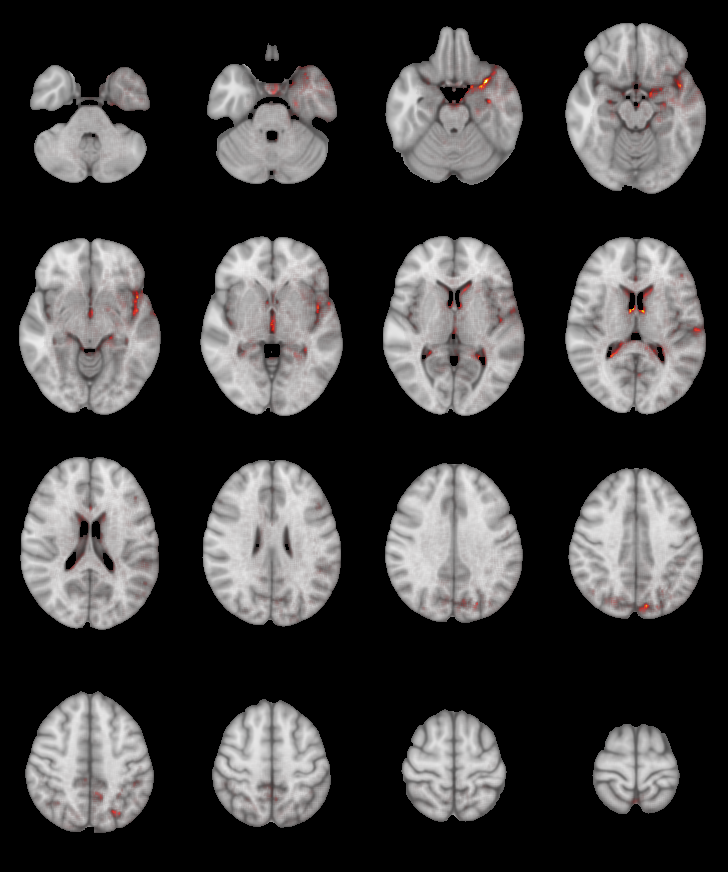
\includegraphics[width=0.31\textwidth]{data/subject1.png}
			};
			\node[anchor=north,inner sep=2pt, text=white, font=\tiny] at (box1.north) {Patient 1};

			\node
				[minimum height=0.41\textwidth,
				minimum width=0.32\textwidth,
				fill=black,
				anchor=west
			] (box2) at ($ (box1.east) + (0.05,0) $) {};
			\node[anchor=south] at (box2.south) {
				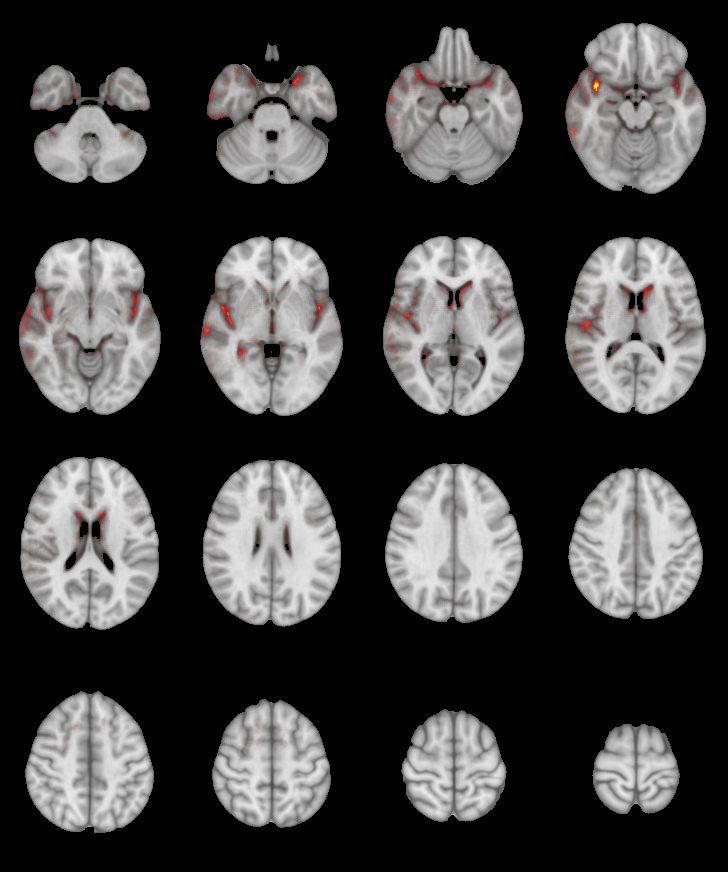
\includegraphics[width=0.31\textwidth]{data/subject2.png}
			};
			\node[anchor=north,inner sep=3pt, text=white, font=\tiny] at (box2.north) {Patient 2};

			\node
				[minimum height=0.41\textwidth,
				minimum width=0.32\textwidth,
				fill=black,
				anchor=west
			] (box3) at ($ (box2.east) + (0.05,0) $) {};
			\node[anchor=south] at (box3.south) {
				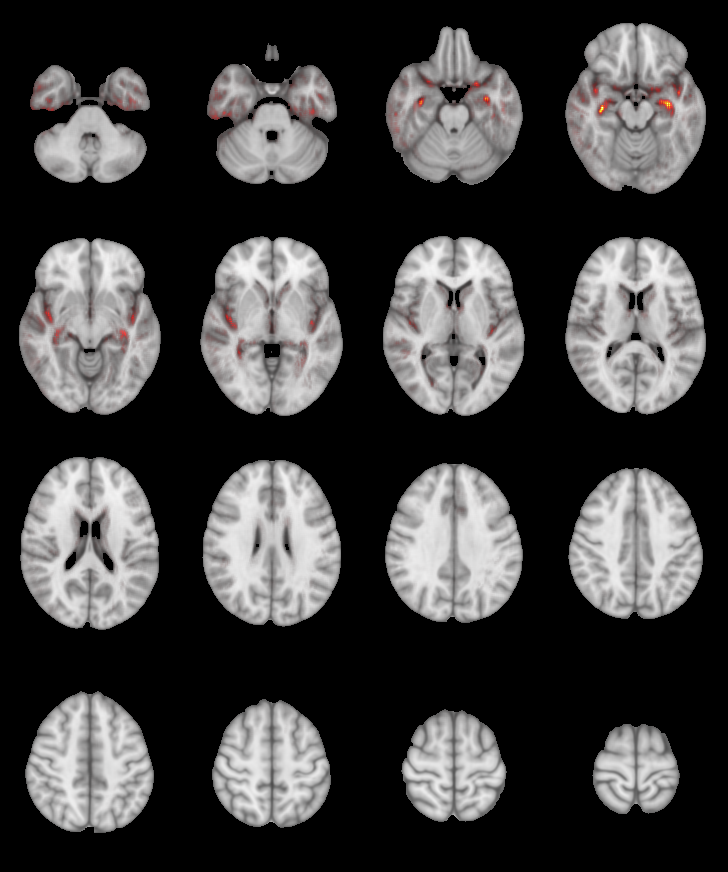
\includegraphics[width=0.31\textwidth]{data/subject3.png}
			};
			\node[anchor=north,inner sep=3pt, text=white, font=\tiny] at (box3.north) {Patient 3};

		\end{tikzpicture}
		\vfill
	\end{frame}


	\begin{frame}{Relevance maps in dementia patients}
		\vfill
		\centering
		\begin{tikzpicture}
			\node[inner sep=0pt, outer sep=0pt, minimum width=3.6cm,label=\tiny{Average dementia patient}] at (0, 0) {
				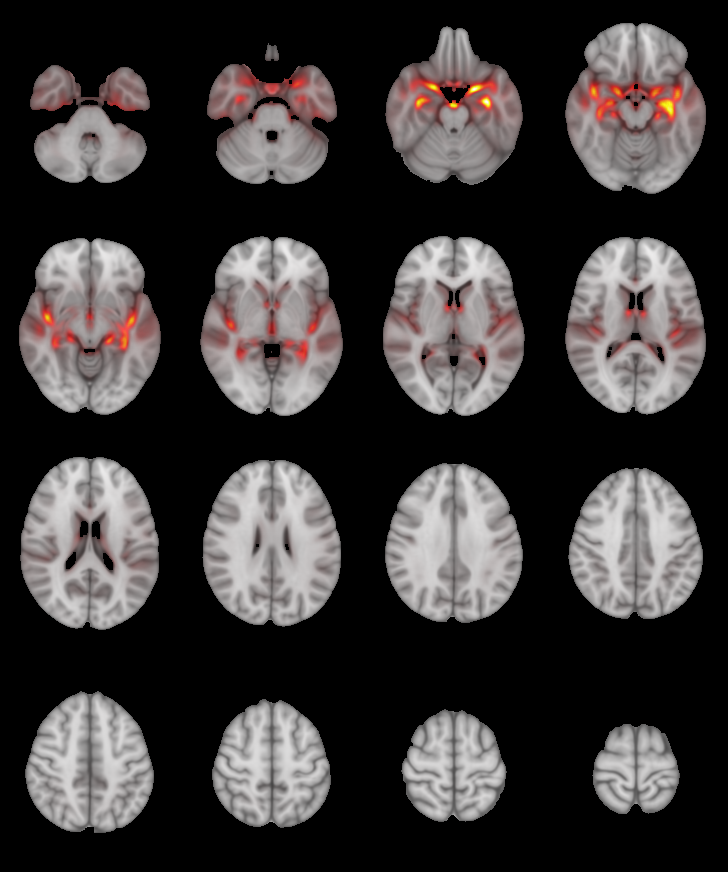
\includegraphics[width=3.6cm]{data/dementia_average.png}
			};

			\node[inner sep=0pt, outer sep=0pt, minimum width=3.6cm] at (3.65, 0) {
			};

			\node[inner sep=0pt, outer sep=0pt, minimum width=3.6cm] at (7.3, 0) {
			};
		\end{tikzpicture}
	\end{frame}

	\begin{frame}{Relevance maps in dementia patients}
		\vfill
		\centering
		\begin{tikzpicture}
			\node[inner sep=0pt, outer sep=0pt, minimum width=3.6cm,label=\tiny{Average dementia patient}] at (0, 0) {
				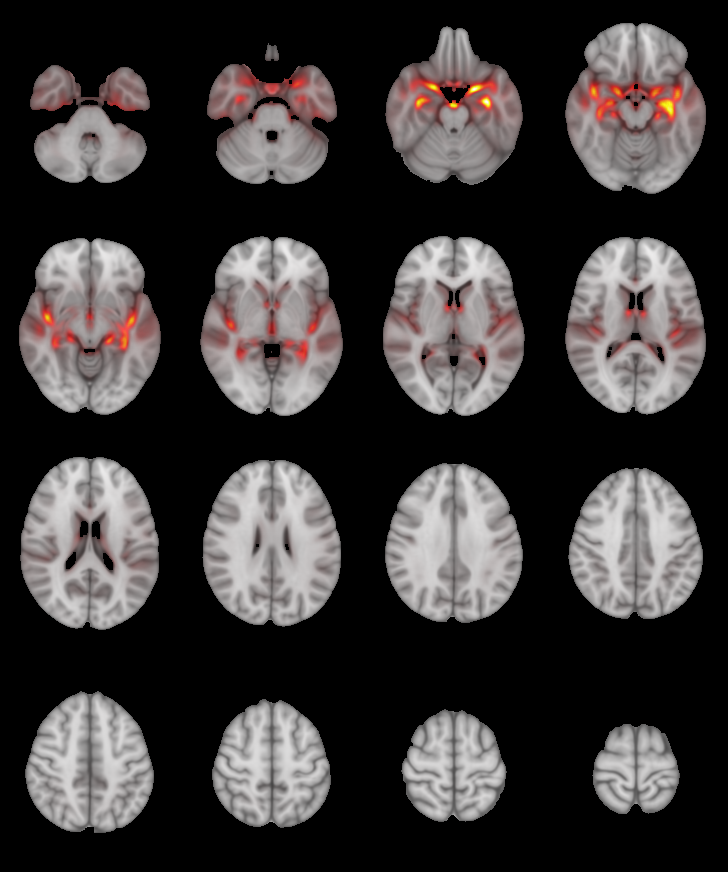
\includegraphics[width=3.6cm]{data/dementia_average.png}
			};

			\node[inner sep=0pt, outer sep=0pt, minimum width=3.6cm,label=\tiny{GingerALE meta-analysis}] at (3.65, 0) {
				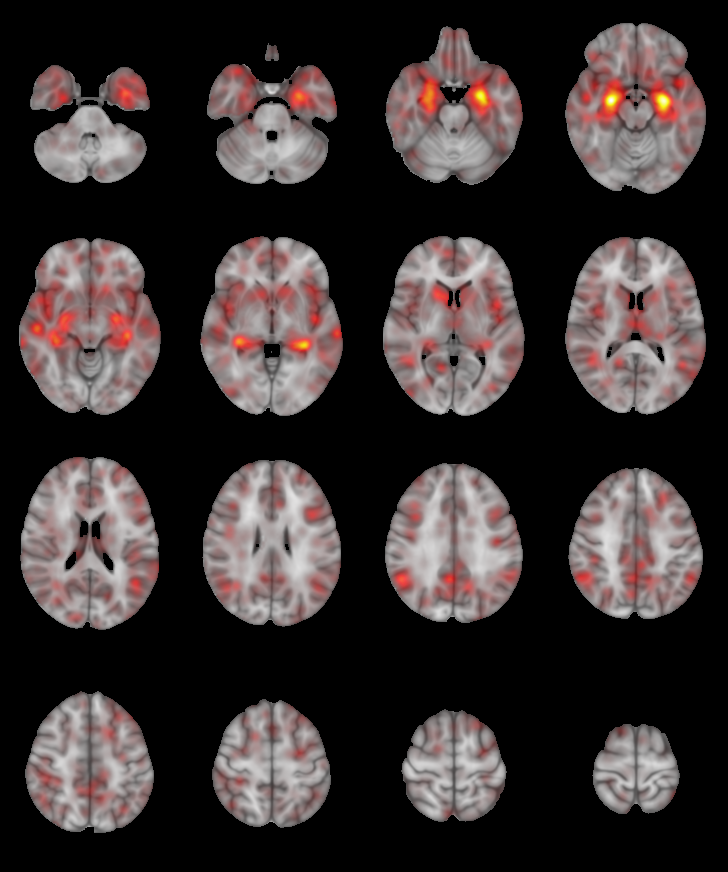
\includegraphics[width=3.6cm]{data/ale.png}
			};

			\node[inner sep=0pt, outer sep=0pt, minimum width=3.6cm] at (7.3, 0) {
			};
		\end{tikzpicture}
	\end{frame}

	\begin{frame}{Relevance maps in dementia patients}
		\vfill
		\centering
		\begin{tikzpicture}
			\node[inner sep=0pt, outer sep=0pt, minimum width=3.6cm,label=\tiny{Average dementia patient}] at (0, 0) {
				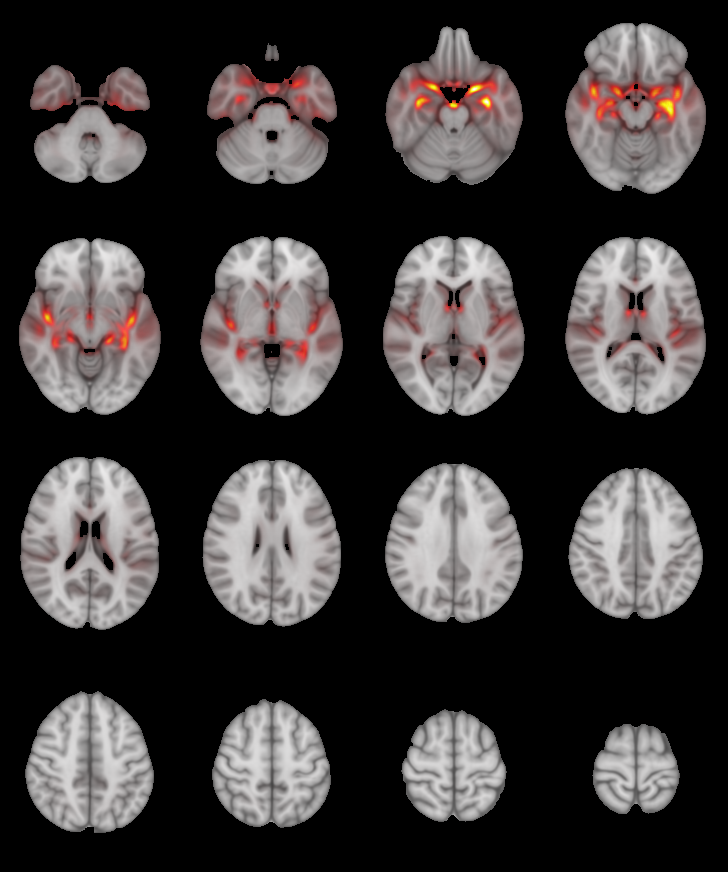
\includegraphics[width=3.6cm]{data/dementia_average.png}
			};

			\node[inner sep=0pt, outer sep=0pt, minimum width=3.6cm,label=\tiny{GingerALE meta-analysis}] at (3.65, 0) {
				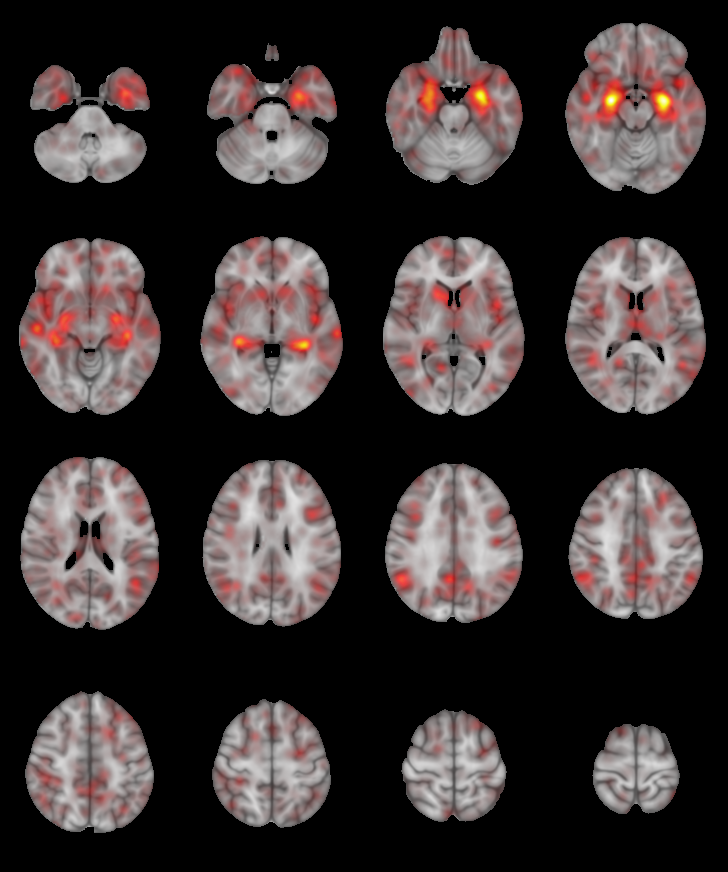
\includegraphics[width=3.6cm]{data/ale.png}
			};

			\node[inner sep=0pt, outer sep=0pt, minimum width=3.6cm,label=\tiny{Overlap}] at (7.3, 0) {
				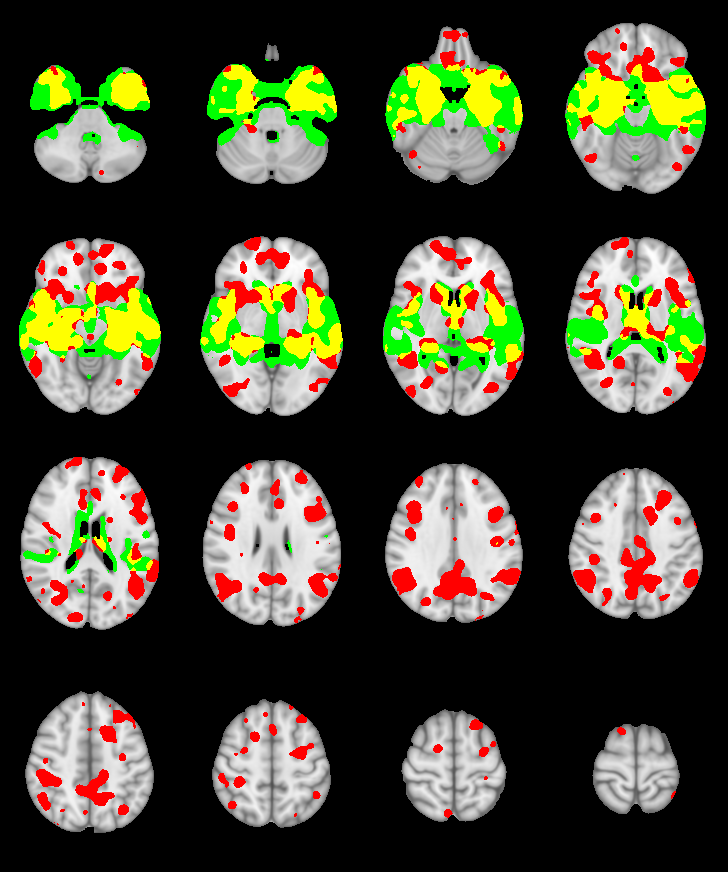
\includegraphics[width=3.6cm]{data/overlap.png}
			};
		\end{tikzpicture}
	\end{frame}
	\vfill

	\begin{frame}{Relevance maps in MCI patients}
		\vfill
		\centering
		\begin{tikzpicture}[scale=0.9]
			\definecolor{controls-default}{HTML}{3594d6}
			\definecolor{cases-default}{HTML}{c71555}

			\colorlet{}{cb-red-purple}
			\colorlet{}{cb-blue}
			\def\xmin{1.15}
			\def\xmax{10.99}
			\def\ymin{-3.5}
			\def\ymax{-0.5}
			\def\xstep{0.492}

			\draw[] (\xmin, \ymax) -- (\xmax, \ymax) -- (\xmax, \ymin) -- (\xmin, \ymin) -- (\xmin, \ymax);
			\node[anchor=east] at (\xmin, -0.5) {\footnotesize{1.0}};
			\node[anchor=east] at (\xmin, -1.1) {\footnotesize{0.8}};
			\node[anchor=east] at (\xmin, -1.7) {\footnotesize{0.6}};
			\node[anchor=east] at (\xmin, -2.3) {\footnotesize{0.4}};
			\node[anchor=east] at (\xmin, -2.9) {\footnotesize{0.2}};
			\node[anchor=east] at (\xmin, -3.5) {\footnotesize{0.0}};
			\node[rotate=90,anchor=south] at ($ (\xmin, -2) - (0.7, 0) $) {\footnotesize{Prediction}};

			\draw[gray!50, thin] (\xmin, -1.1) -- (\xmax, -1.1);
			\draw[gray!50, thin] (\xmin, -1.7) -- (\xmax, -1.7);
			\draw[gray!50, thin] (\xmin, -2.3) -- (\xmax, -2.3);
			\draw[gray!50, thin] (\xmin, -2.9) -- (\xmax, -2.9);

			\newcommand{\prediction}[4]{
				\node[circle, inner sep=0pt, outer sep=0pt, minimum size=6pt, draw=black, fill=####3] (####4) at (\xmin + ####1 * \xstep, \ymin+3*####2) {};
			}

			\prediction{1}{0.5369713}{controls-default}{p1}
			\prediction{3}{0.5685464}{controls-default}{p2}
			\prediction{5}{0.72608125}{cases-default}{p3}
			\prediction{7}{0.7650767}{cases-default}{p4}
			\prediction{9}{0.78441274}{cases-default}{p5}
			\prediction{11}{0.77807206}{cases-default}{p6}
			\prediction{13}{0.96812713}{cases-default}{p7}
			\prediction{15}{0.9813527}{cases-default}{p8}
			\prediction{17}{0.99700356}{cases-default}{p9}
			\prediction{19}{0.998078}{cases-default}{p10}

			\draw[controls-default, thick] (p1) -- (p2) -- (p3);
			\draw[cases-default, thick] (p3) -- (p4) -- (p5) -- (p6) -- (p7) -- (p8) -- (p9) -- (p10);

			\draw[fill=black] (\xmin, \ymin) -- (\xmax, \ymin) -- (\xmax, \ymin - 5.1) -- (\xmin, \ymin - 5.1) -- (\xmin, \ymin);

			\node[anchor=north, inner sep=0pt, outer sep=0pt] at (\xmin + 10*\xstep+0.001, \ymin - 0.2) {
				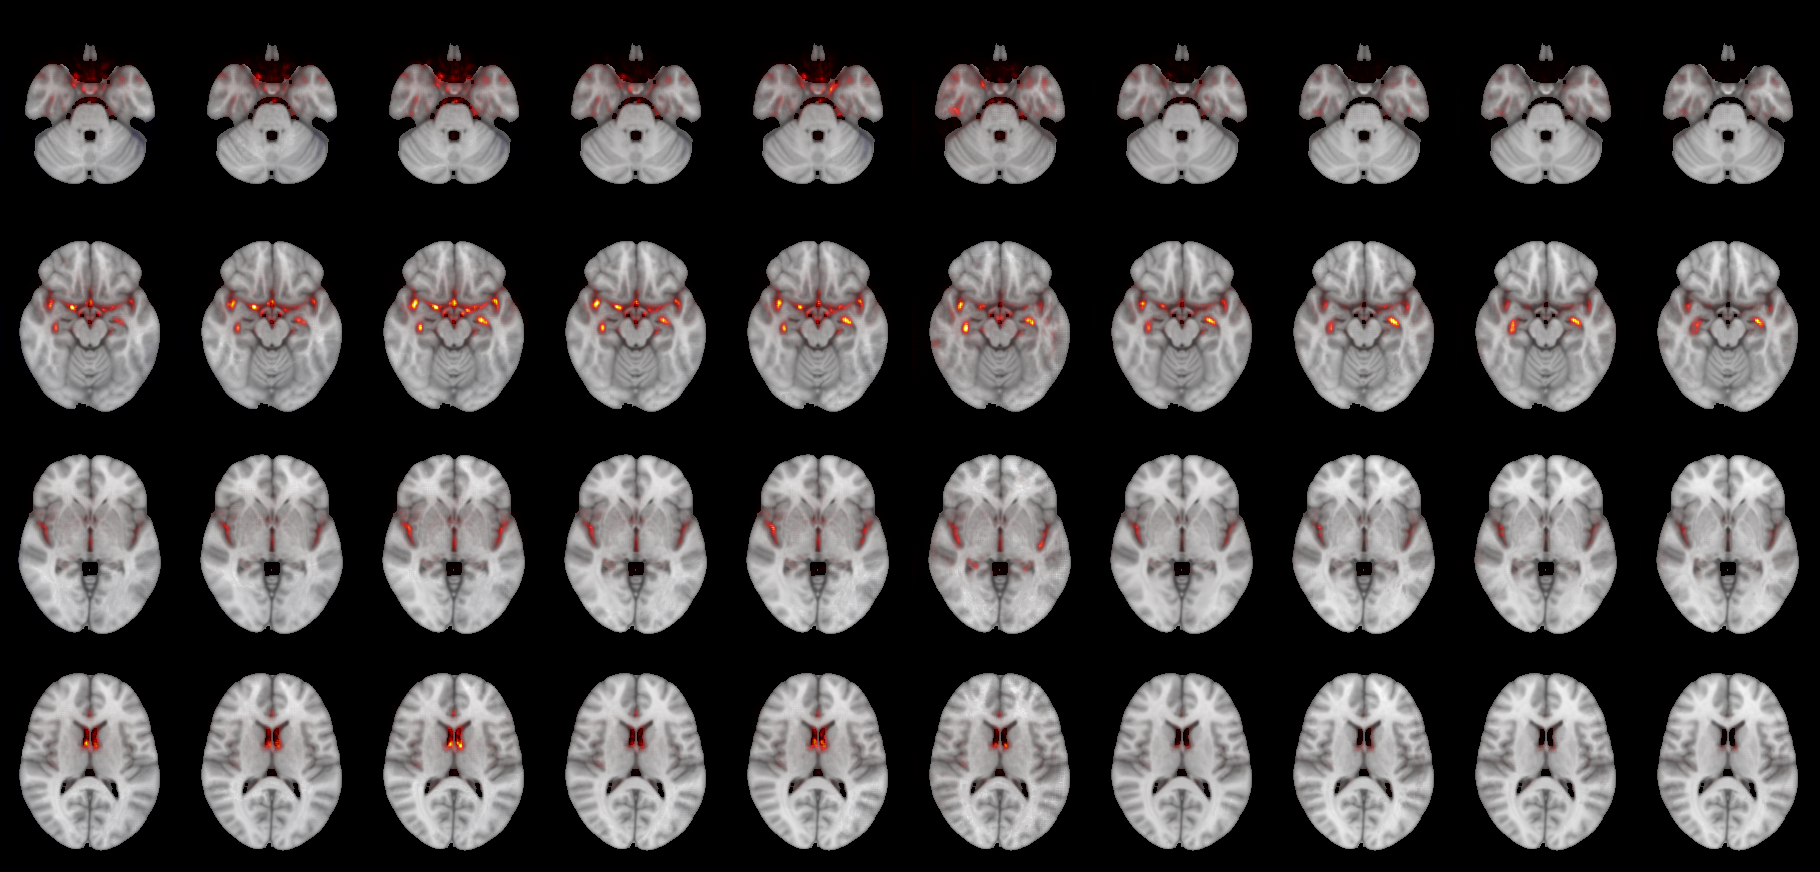
\includegraphics[width=0.82\textwidth]{data/MCI_to_AD.png}
			};

			\newcommand{\datenode}[2]{
				\node[fill=black,inner sep=0pt,anchor=north,font=\tiny\selectfont] at ($ (\xmin, \ymin) + (####2 * \xstep, -0.1) $) {\textcolor{white}{####1}};
			}

			\datenode{17.07.06}{1}
			\datenode{22.02.07}{3}
			\datenode{05.09.07}{5}
			\datenode{03.04.08}{7}
			\datenode{29.09.08}{9}
			\datenode{13.08.09}{11}
			\datenode{22.07.10}{13}
			\datenode{16.08.11}{15}
			\datenode{07.08.12}{17}
			\datenode{16.08.13}{19}

		\end{tikzpicture}
		\vfill
	\end{frame}

	\begin{frame}{Relevance maps in MCI patients}
		\vfill
		\centering
		\begin{tikzpicture}[scale=0.9]
			\definecolor{controls-default}{HTML}{3594d6}
			\definecolor{cases-default}{HTML}{c71555}

			\colorlet{}{cb-red-purple}
			\colorlet{}{cb-blue}
			\def\xmin{1.15}
			\def\xmax{7.05}
			\def\ymin{-3.5}
			\def\ymax{-0.5}
			\def\xstep{0.492}

			\draw[] (\xmin, \ymax) -- (\xmax, \ymax) -- (\xmax, \ymin) -- (\xmin, \ymin) -- (\xmin, \ymax);
			\node[anchor=east] at (\xmin, -0.5) {\footnotesize{1.0}};
			\node[anchor=east] at (\xmin, -1.1) {\footnotesize{0.8}};
			\node[anchor=east] at (\xmin, -1.7) {\footnotesize{0.6}};
			\node[anchor=east] at (\xmin, -2.3) {\footnotesize{0.4}};
			\node[anchor=east] at (\xmin, -2.9) {\footnotesize{0.2}};
			\node[anchor=east] at (\xmin, -3.5) {\footnotesize{0.0}};
			\node[rotate=90,anchor=south] at ($ (\xmin, -2) - (0.7, 0) $) {\footnotesize{Prediction}};

			\draw[gray!50, thin] (\xmin, -1.1) -- (\xmax, -1.1);
			\draw[gray!50, thin] (\xmin, -1.7) -- (\xmax, -1.7);
			\draw[gray!50, thin] (\xmin, -2.3) -- (\xmax, -2.3);
			\draw[gray!50, thin] (\xmin, -2.9) -- (\xmax, -2.9);

			\newcommand{\prediction}[4]{
				\node[circle, inner sep=0pt, outer sep=0pt, minimum size=6pt, draw=black, fill=####3] (####4) at (\xmin + ####1 * \xstep, \ymin+3*####2) {};
			}

			\prediction{1}{0.8506671}{controls-default}{p1}
			\prediction{3}{0.73082274}{controls-default}{p2}
			\prediction{5}{0.757359946}{controls-default}{p3}
			\prediction{7}{0.83361979}{controls-default}{p4}
			\prediction{9}{0.890486}{controls-default}{p5}
			\prediction{11}{0.894983}{controls-default}{p6}

			\draw[controls-default, thick] (p1) -- (p2) -- (p3) -- (p4) -- (p5) -- (p6);

			\draw[fill=black] (\xmin, \ymin) -- (\xmax, \ymin) -- (\xmax, \ymin - 5.1) -- (\xmin, \ymin - 5.1) -- (\xmin, \ymin);

			\node[anchor=north, inner sep=0pt, outer sep=0pt] at (\xmin + 6*\xstep+0.001, \ymin - 0.2) {
				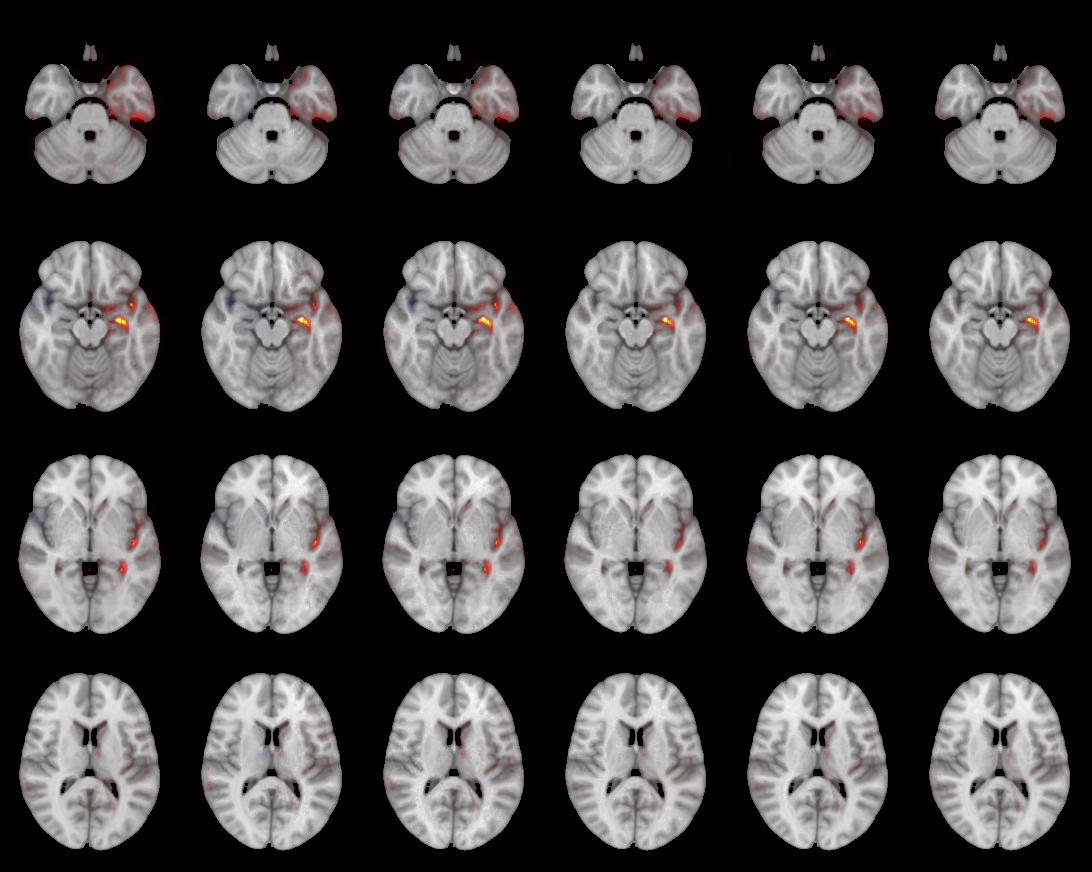
\includegraphics[width=0.49\textwidth]{data/MCI.png}
			};

			\newcommand{\datenode}[2]{
				\node[fill=black,inner sep=0pt,anchor=north,font=\tiny\selectfont] at ($ (\xmin, \ymin) + (####2 * \xstep, -0.1) $) {\textcolor{white}{####1}};
			}

			\datenode{14.08.06}{1}
			\datenode{11.04.07}{3}
			\datenode{19.09.07}{5}
			\datenode{18.06.08}{7}
			\datenode{17.10.08}{9}
			\datenode{04.09.09}{11}

		\end{tikzpicture}
		\vfill
	\end{frame}

	\begin{frame}{Relevance maps in MCI patients}
		\vfill
		\centering
		\begin{tikzpicture}[scale=0.9]
			\definecolor{controls-default}{HTML}{3594d6}
			\definecolor{cases-default}{HTML}{c71555}
			\definecolor{healthy-default}{HTML}{4dac93}
			\def\xmin{1.15}
			\def\xmax{8.03}
			\def\ymin{-3.5}
			\def\ymax{-0.5}
			\def\xstep{0.492}

			\draw[] (\xmin, \ymax) -- (\xmax, \ymax) -- (\xmax, \ymin) -- (\xmin, \ymin) -- (\xmin, \ymax);
			\node[anchor=east] at (\xmin, -0.5) {\footnotesize{1.0}};
			\node[anchor=east] at (\xmin, -1.1) {\footnotesize{0.8}};
			\node[anchor=east] at (\xmin, -1.7) {\footnotesize{0.6}};
			\node[anchor=east] at (\xmin, -2.3) {\footnotesize{0.4}};
			\node[anchor=east] at (\xmin, -2.9) {\footnotesize{0.2}};
			\node[anchor=east] at (\xmin, -3.5) {\footnotesize{0.0}};
			\node[rotate=90,anchor=south] at ($ (\xmin, -2) - (0.7, 0) $) {\footnotesize{Prediction}};

			\draw[gray!50, thin] (\xmin, -1.1) -- (\xmax, -1.1);
			\draw[gray!50, thin] (\xmin, -1.7) -- (\xmax, -1.7);
			\draw[gray!50, thin] (\xmin, -2.3) -- (\xmax, -2.3);
			\draw[gray!50, thin] (\xmin, -2.9) -- (\xmax, -2.9);

			\newcommand{\prediction}[4]{
				\node[circle, inner sep=0pt, outer sep=0pt, minimum size=6pt, draw=black, fill=####3] (####4) at (\xmin + ####1 * \xstep, \ymin+3*####2) {};
			}



			\draw[fill=black] (\xmin, \ymin) -- (\xmax, \ymin) -- (\xmax, \ymin - 5.1) -- (\xmin, \ymin - 5.1) -- (\xmin, \ymin);

			\node[anchor=north, inner sep=0pt, outer sep=0pt] at (\xmin + 7*\xstep+0.001, \ymin - 0.2) {
				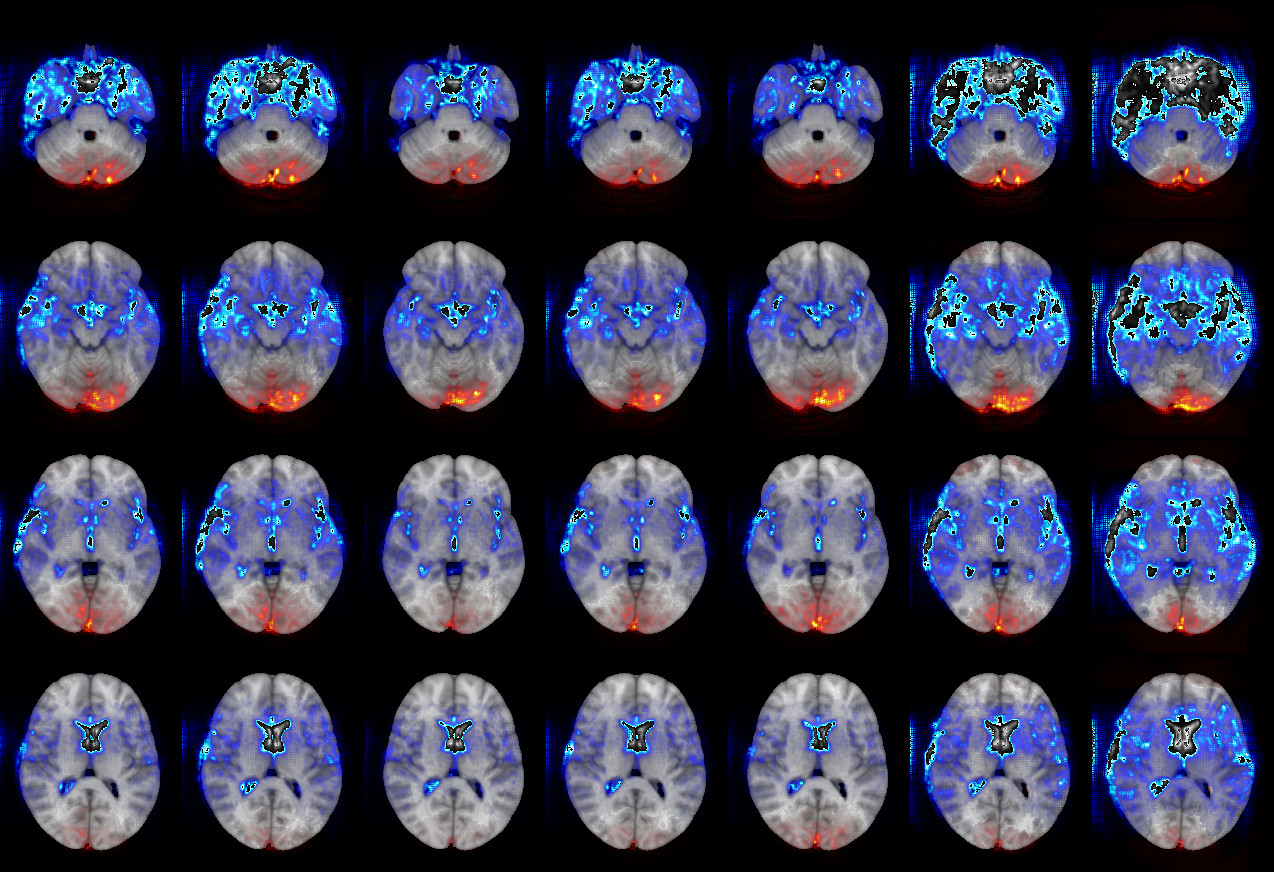
\includegraphics[width=0.57\textwidth]{data/MCI_to_CN.png}
			};

			\newcommand{\datenode}[2]{
				\node[fill=black,inner sep=0pt,anchor=north,font=\tiny\selectfont] at ($ (\xmin, \ymin) + (####2 * \xstep, -0.1) $) {\textcolor{white}{####1}};
			}

			\datenode{24.06.10}{1}
			\datenode{22.10.10}{3}
			\datenode{22.01.11}{5}
			\datenode{07.07.11}{7}
			\datenode{11.07.12}{9}
			\datenode{18.07.13}{11}
			\datenode{13.08.15}{13}

			\prediction{1}{0.040251}{controls-default}{p1}
			\prediction{3}{0.032405}{controls-default}{p2}
			\prediction{5}{0.036456}{healthy-default}{p3}
			\prediction{7}{0.0369694}{healthy-default}{p4}
			\prediction{9}{0.03886}{healthy-default}{p5}
			\prediction{11}{0.0409125}{healthy-default}{p6}
			\prediction{13}{0.036031}{healthy-default}{p7}

			\draw[controls-default, thick] (p1) -- (p2) -- (p3);
			\draw[healthy-default, thick] (p3) -- (p4) -- (p5) -- (p6) -- (p7);

		\end{tikzpicture}
		\vfill
	\end{frame}

	\begin{frame}{Relevance maps in MCI patients}
		\vfill
		\begin{tikzpicture}
			\definecolor{controls-default}{HTML}{3594d6}
			\definecolor{cases-default}{HTML}{c71555}
			\definecolor{healthy-default}{HTML}{4dac93}

			\begin{axis}[
				width=0.84\textwidth,
				height=0.7\textwidth,
				xmin=-12,
				xmax=0,
				ymin=-0.05,
				ymax=1.05,
				ylabel=Prediction,
				every tick label/.append style={font=\footnotesize},
				xlabel={Years to diagnosis},
				clip=false,
				grid,
				grid style={line width=0.05mm, gray!50},
				xtick style={draw=none},
				ytick style={draw=none}
			]
				\addplot[mark=*,mark options={fill=cases-default}] table [
					x expr=\thisrow{bucket} * -3 / 12,
					y=mean,
					col sep=comma
				] {data/patient_histories.csv};
				\addplot[mark=*,mark options={fill=controls-default}] table [
					x expr=\thisrow{bucket} * -3 / 12,
					y=mean,
					col sep=comma
				] {data/control_histories.csv};
			\end{axis}
		\end{tikzpicture}
		\vfill
	\end{frame}

	\begin{frame}{Relevance maps in MCI patients}
		\vfill
		\begin{tikzpicture}
			\definecolor{controls-default}{HTML}{3594d6}
			\definecolor{cases-default}{HTML}{c71555}
			\definecolor{healthy-default}{HTML}{4dac93}

			\begin{axis}[
				width=0.84\textwidth,
				height=0.7\textwidth,
				xmin=-12,
				xmax=0,
				ymin=-0.05,
				ymax=1.05,
				ylabel=Prediction,
				every tick label/.append style={font=\footnotesize},
				xlabel={Years to diagnosis},
				clip=false,
				grid,
				grid style={line width=0.05mm, gray!50},
				xtick style={draw=none},
				ytick style={draw=none}
			]
				\addplot[mark=*,mark options={fill=cases-default}] table [
					x expr=\thisrow{bucket} * -3 / 12,
					y=mean,
					col sep=comma
				] {data/patient_histories.csv};
				\addplot[mark=*,mark options={fill=controls-default}] table [
					x expr=\thisrow{bucket} * -3 / 12,
					y=mean,
					col sep=comma
				] {data/control_histories.csv};
				\addplot[cases-default, dashed] coordinates {
					(-12, 0.677)
					(0, 0.677)
				} node[anchor=west] at (axis cs: 0, 0.677) {\scriptsize{0.677}};
				\addplot[controls-default, dashed] coordinates {
					(-12, 0.304)
					(0, 0.304)
				} node[anchor=west] at (axis cs: 0, 0.304) {\scriptsize{0.304}};
				\draw[Latex-Latex, thick, densely dotted] (axis cs: -0.2, 0.304) -- (axis cs: -0.2, 0.677);
				\coordinate (coef) at (axis cs: 0, 0.490);
			\end{axis}
			\node[anchor=west,align=left,font=\scriptsize\linespread{0.8}\selectfont] at (coef) {$\beta\mathrm{=}0.441$\\$p\mathrm{=}4.87 * 10^{-60}$};
		\end{tikzpicture}
		\vfill
	\end{frame}

	\begin{frame}{Relevance maps in MCI patients}
		\vfill
		\begin{tikzpicture}
			\definecolor{controls-default}{HTML}{3594d6}
			\definecolor{cases-default}{HTML}{c71555}
			\definecolor{healthy-default}{HTML}{4dac93}

			\begin{axis}[
				width=0.84\textwidth,
				height=0.7\textwidth,
				xmin=-12,
				xmax=0,
				ymin=-0.05,
				ymax=1.05,
				ylabel=Prediction,
				every tick label/.append style={font=\footnotesize},
				xlabel={Years to diagnosis},
				clip=false,
				grid,
				grid style={line width=0.05mm, gray!50},
				xtick style={draw=none},
				ytick style={draw=none}
			]
				\addplot[mark=*,mark options={fill=cases-default}] table [
					x expr=\thisrow{bucket} * -3 / 12,
					y=mean,
					col sep=comma
				] {data/patient_histories.csv};
				\addplot[mark=*,mark options={fill=controls-default}] table [
					x expr=\thisrow{bucket} * -3 / 12,
					y=mean,
					col sep=comma
				] {data/control_histories.csv};
				\addplot[dashed] coordinates {
					(-12, 0.677)
					(0, 0.677)
				};
				\addplot[dashed] coordinates {
					(-12, 0.304)
					(0, 0.304)
				};
				\addplot[cases-default, dashed] coordinates {
					(-12, 0.42)
					(0, 0.73)
				};
				\addplot[controls-default, dashed] coordinates {
					(-10, 0.10)
					(0, 0.34)
				};
				\draw[Latex-Latex, thick, densely dotted] (axis cs: -0.2, 0.337) -- (axis cs: -0.2, 0.727);
				\coordinate (coef) at (axis cs: 0, 0.532);
			\end{axis}
			\node[anchor=west,align=left,font=\scriptsize\linespread{0.8}\selectfont] at (coef) {$\beta\mathrm{=}0.047$\\$p\mathrm{=}6.12 * 10^{-15}$};
		\end{tikzpicture}
		\vfill
	\end{frame}

	\begin{frame}{Relevance maps in MCI patients}
		\vfill
		\centering
		\begin{tikzpicture}
			\node[] at (0, 0) {
				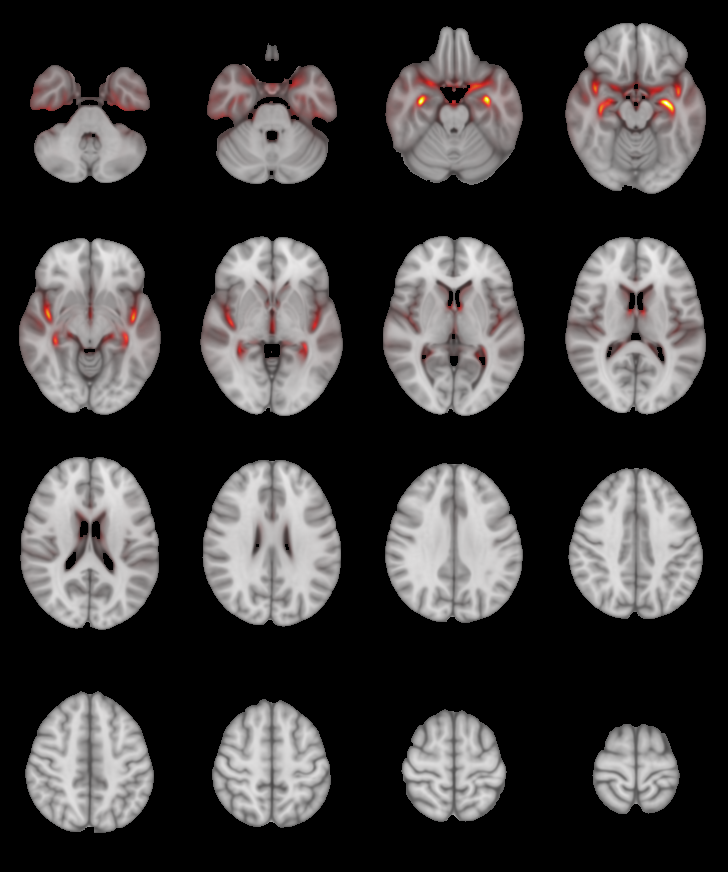
\includegraphics[width=2.5cm]{data/component_0.png}
			};
			\node[] at (2.55, 0) {
				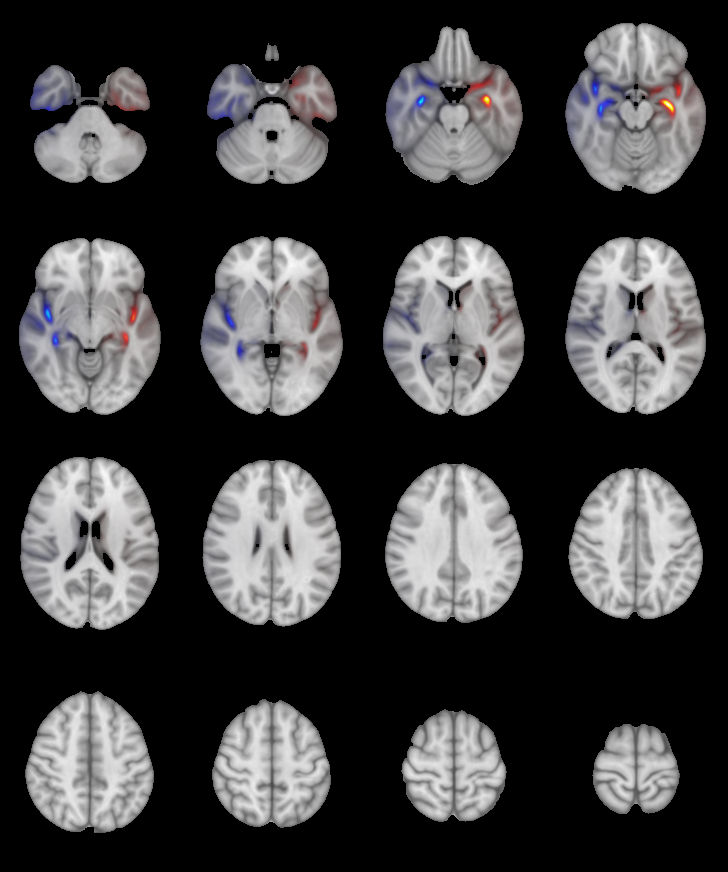
\includegraphics[width=2.5cm]{data/component_1.png}
			};
			\node[] at (5.1, 0) {
				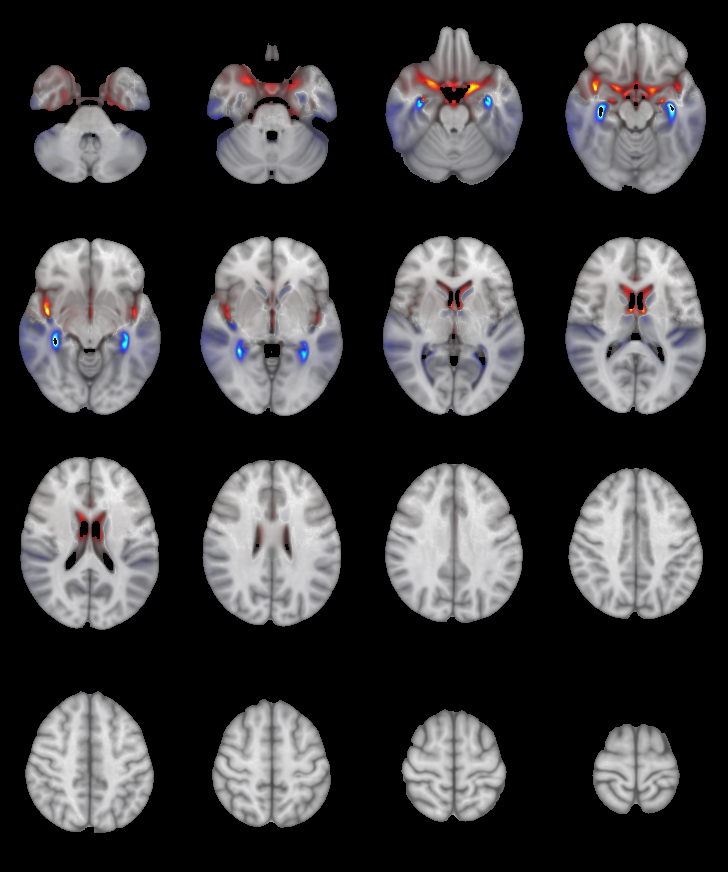
\includegraphics[width=2.5cm]{data/component_2.png}
			};
			\node[] at (7.65, 0) {
				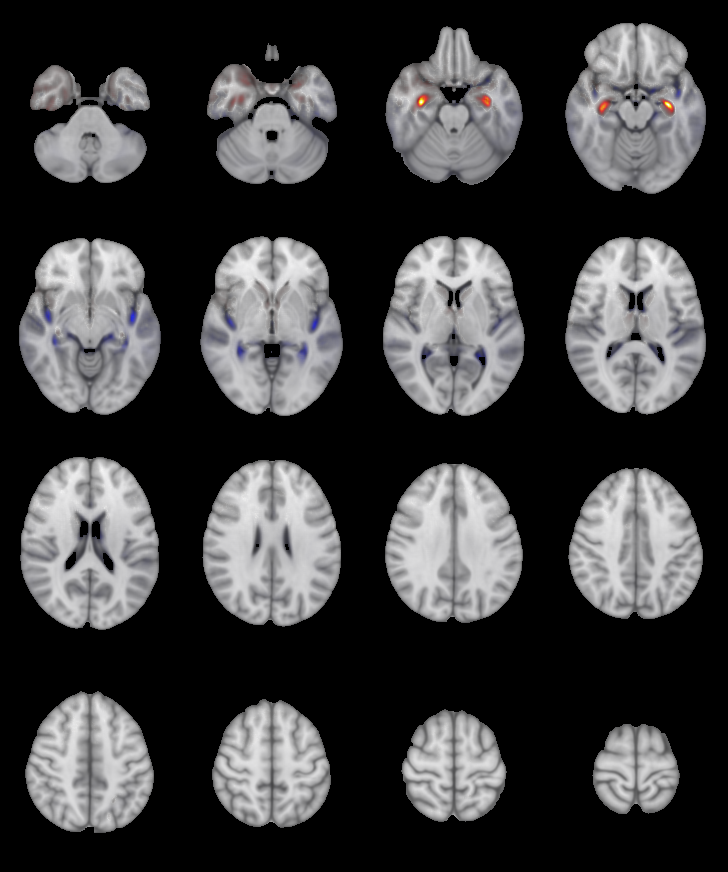
\includegraphics[width=2.5cm]{data/component_3.png}
			};
			\node[] at (0, -4) {};
		\end{tikzpicture}
		\vfill
	\end{frame}

	\begin{frame}{Relevance maps in MCI patients}
		\vfill
		\centering
		\begin{tikzpicture}
			\definecolor{controls-default}{HTML}{3594d6}

			\node[] at (0, 0) {
				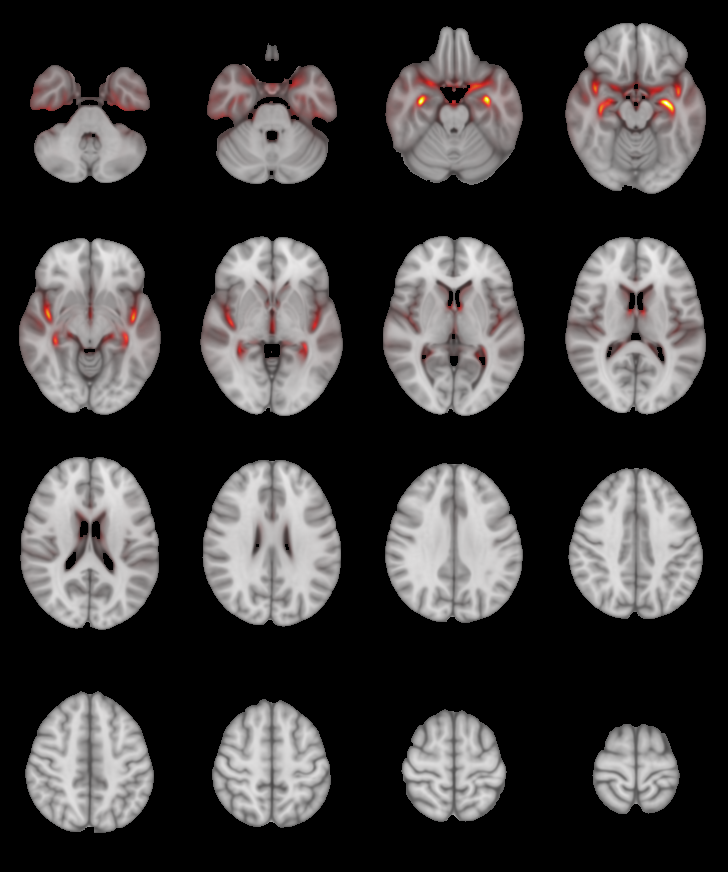
\includegraphics[width=2.5cm]{data/component_0.png}
			};
			\node[] at (2.55, 0) {
				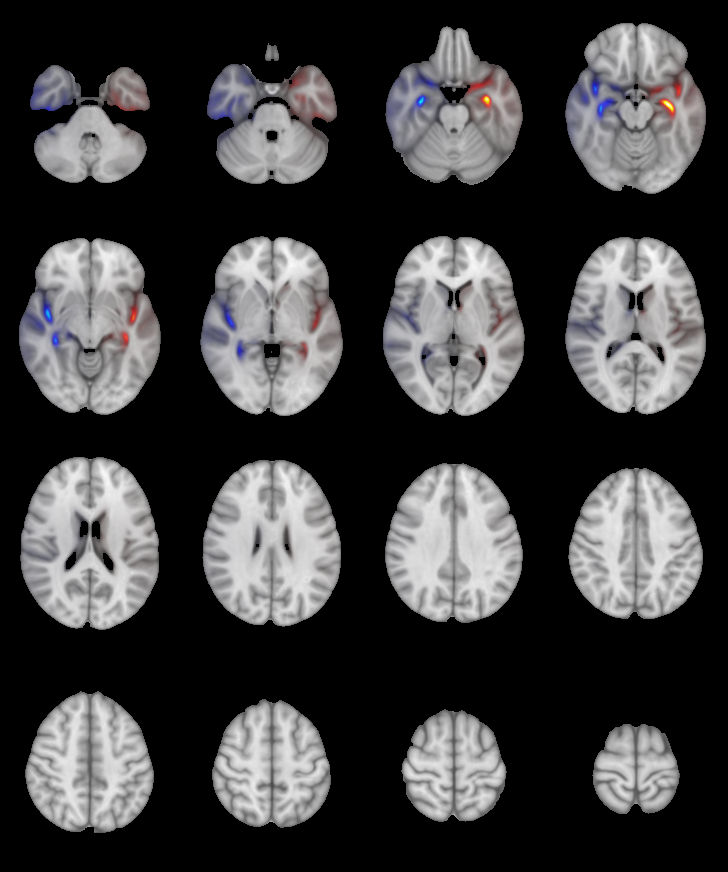
\includegraphics[width=2.5cm]{data/component_1.png}
			};
			\node[] at (5.1, 0) {
				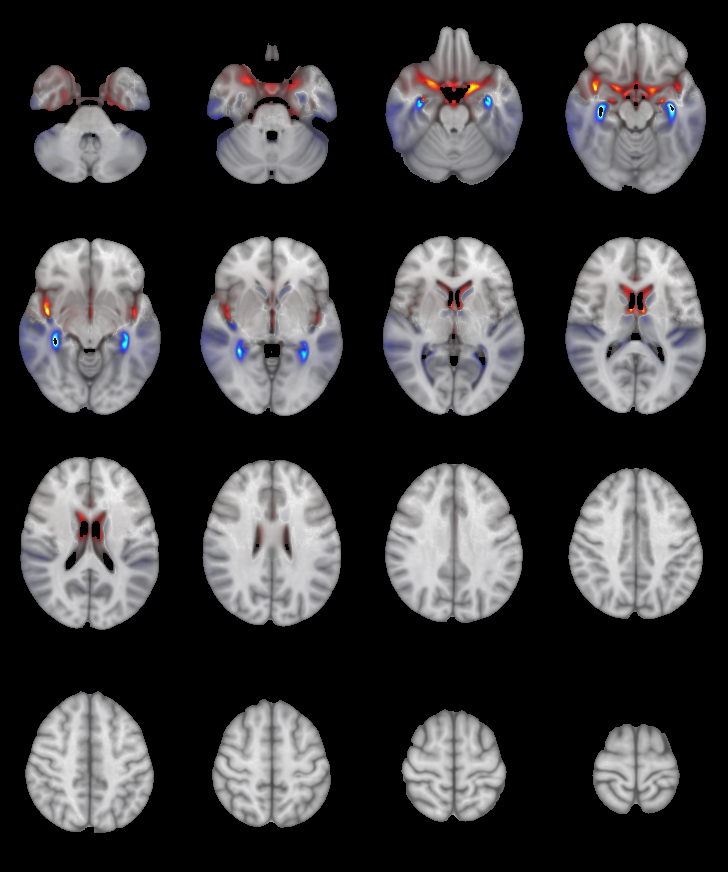
\includegraphics[width=2.5cm]{data/component_2.png}
			};
			\node[] at (7.65, 0) {
				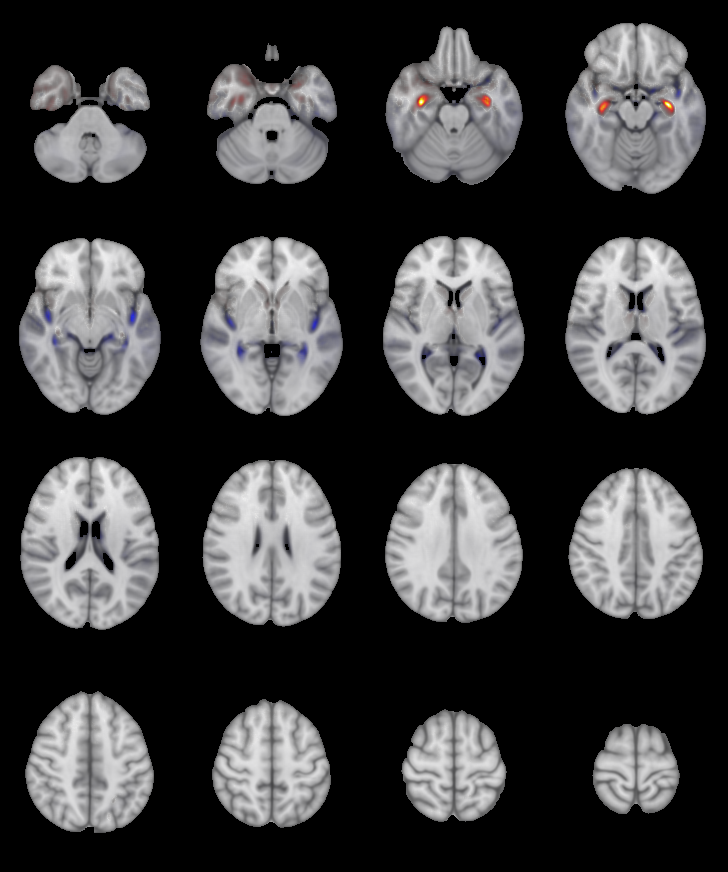
\includegraphics[width=2.5cm]{data/component_3.png}
			};
			\node[] at (0, -4) {};

			\draw[Latex-Latex, very thick] (0, -3.5) -- (7.65, -3.5);
			\draw[very thick] (3.825,-3.575) -- (3.825,-3.425);
			\node[anchor=north] at (3.825,-3.55) {\footnotesize{0}};
			\node[anchor=west] at (7.65,-3.5) {\footnotesize{\textbf{+}}};
			\node[anchor=east] at (0,-3.5) {\footnotesize{\textbf{-}}};
		\end{tikzpicture}
		\vfill
	\end{frame}

	\begin{frame}{Relevance maps in MCI patients}
		\vfill
		\centering
		\begin{tikzpicture}
			\definecolor{controls-default}{HTML}{3594d6}

			\node[] at (0, 0) {
				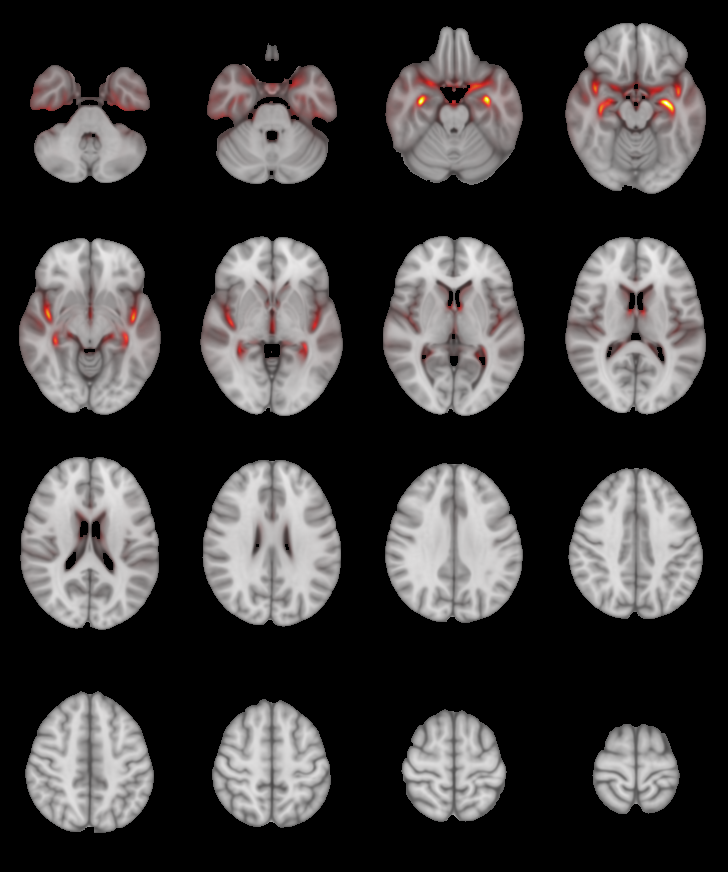
\includegraphics[width=2.5cm]{data/component_0.png}
			};
			\node[] at (2.55, 0) {
				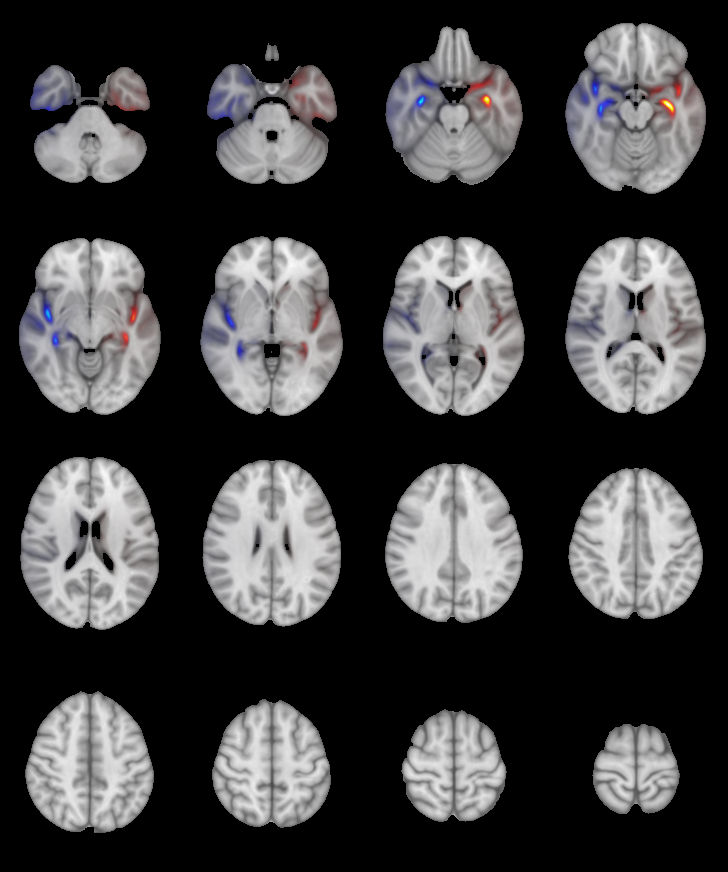
\includegraphics[width=2.5cm]{data/component_1.png}
			};
			\node[] at (5.1, 0) {
				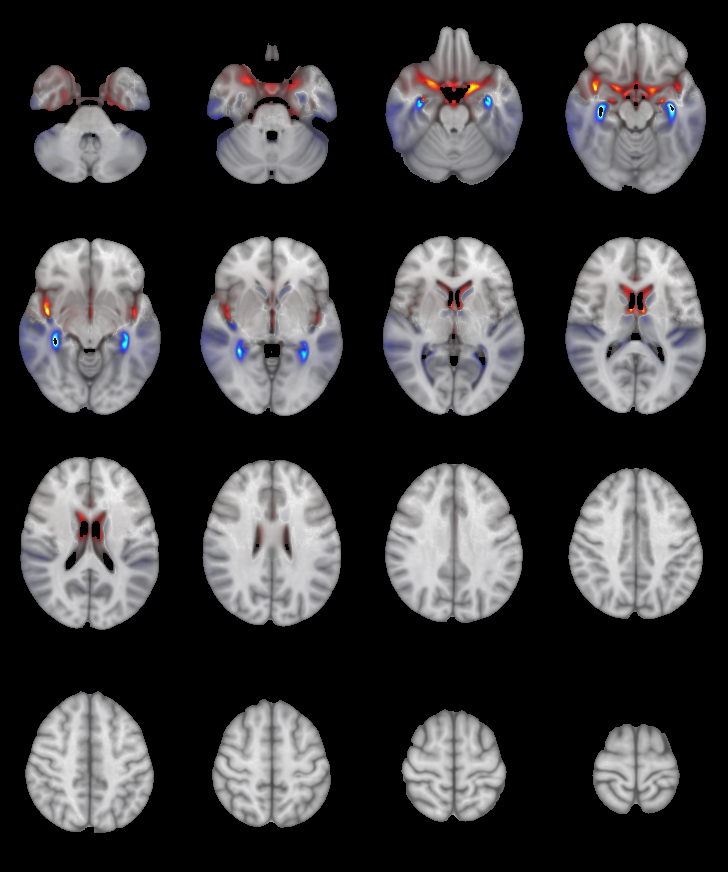
\includegraphics[width=2.5cm]{data/component_2.png}
			};
			\node[] at (7.65, 0) {
				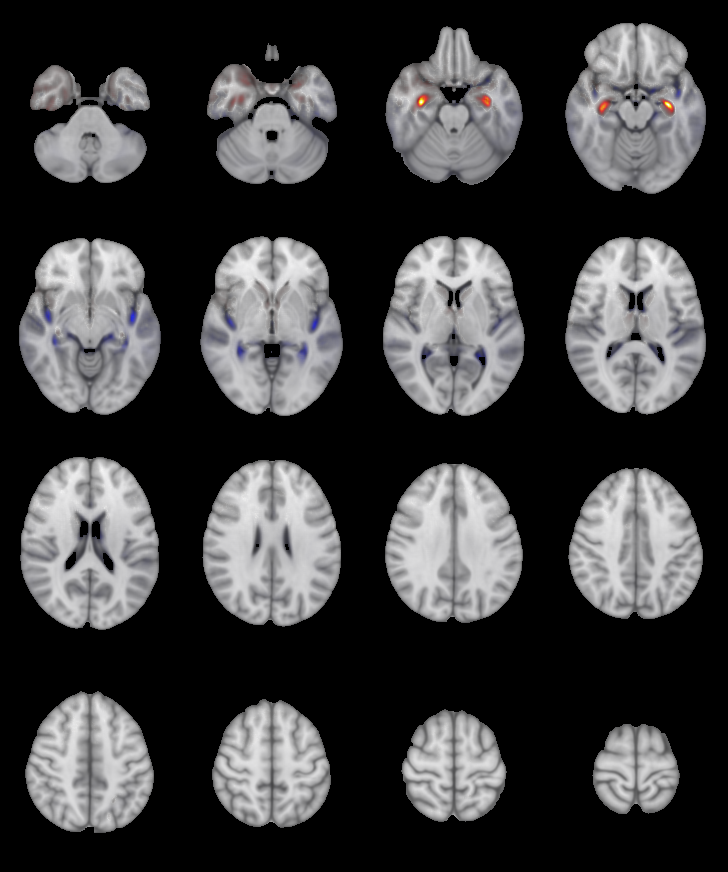
\includegraphics[width=2.5cm]{data/component_3.png}
			};
			\node[] at (0, -4) {};

			\draw[Latex-Latex, very thick] (0, -3.5) -- (7.65, -3.5);
			\draw[very thick] (3.825,-3.575) -- (3.825,-3.425);
			\node[anchor=north] at (3.825,-3.55) {\footnotesize{0}};
			\node[anchor=west] at (7.65,-3.5) {\footnotesize{\textbf{+}}};
			\node[anchor=east] at (0,-3.5) {\footnotesize{\textbf{-}}};
			\node[circle,draw=black,fill=controls-default,inner sep=2pt] (pos) at (6.5,-3.5) {};
			\node[anchor=south] at (pos.north) {
				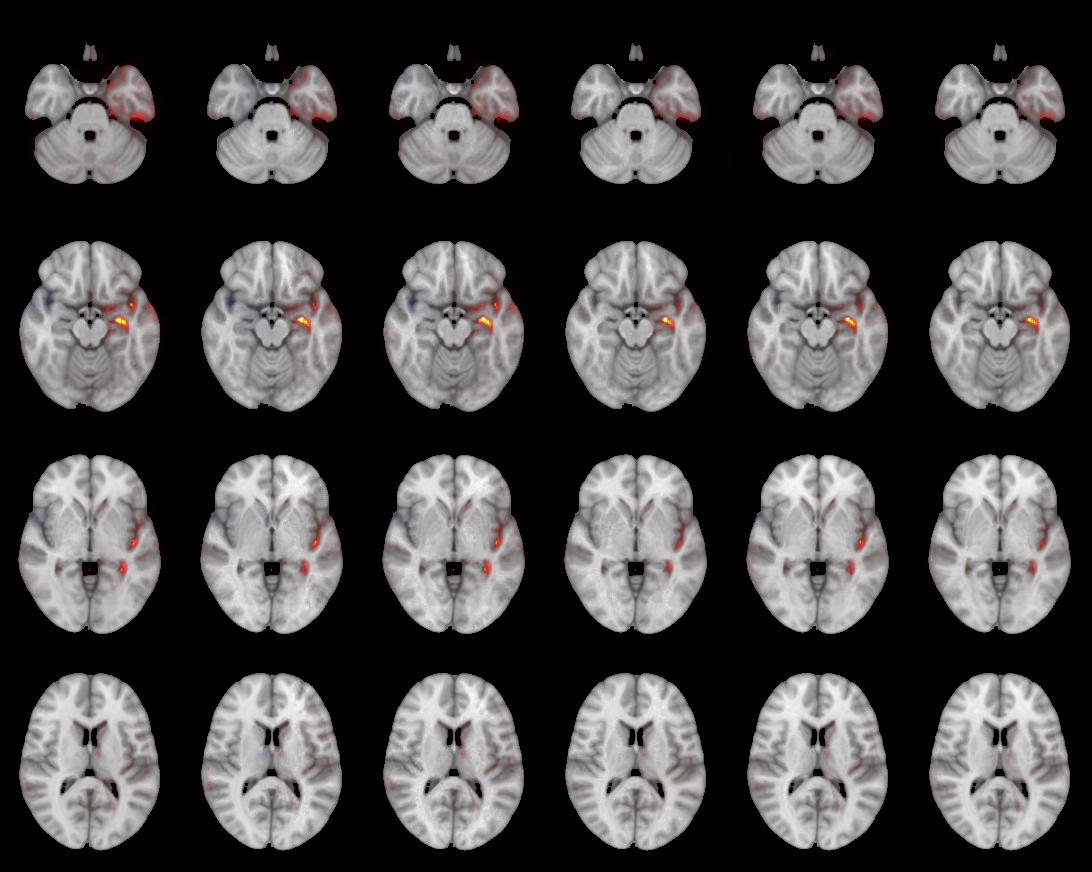
\includegraphics[
					width=1.2cm,
					clip=true,
					trim = 319mm 150mm 0mm 75mm
				]{data/MCI.png}
			};
		\end{tikzpicture}
		\vfill
	\end{frame}

	\begin{frame}{Relevance maps in MCI patients}
		\vfill
		\centering
		\begin{tikzpicture}
			\definecolor{controls-default}{HTML}{3594d6}

			\node[] at (0, 0) {
				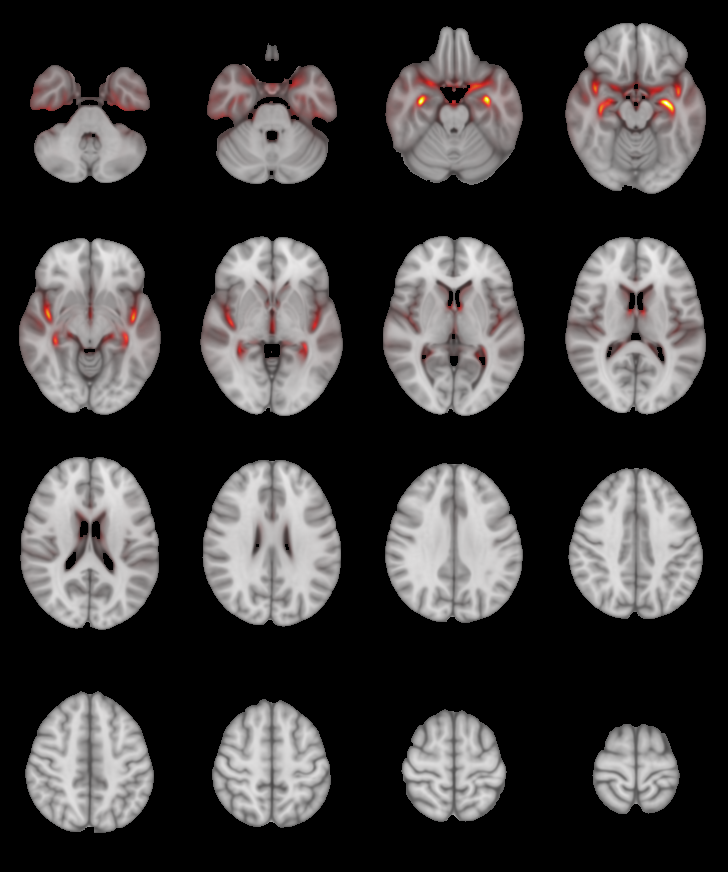
\includegraphics[width=2.5cm]{data/component_0.png}
			};
			\node[] at (2.55, 0) {
				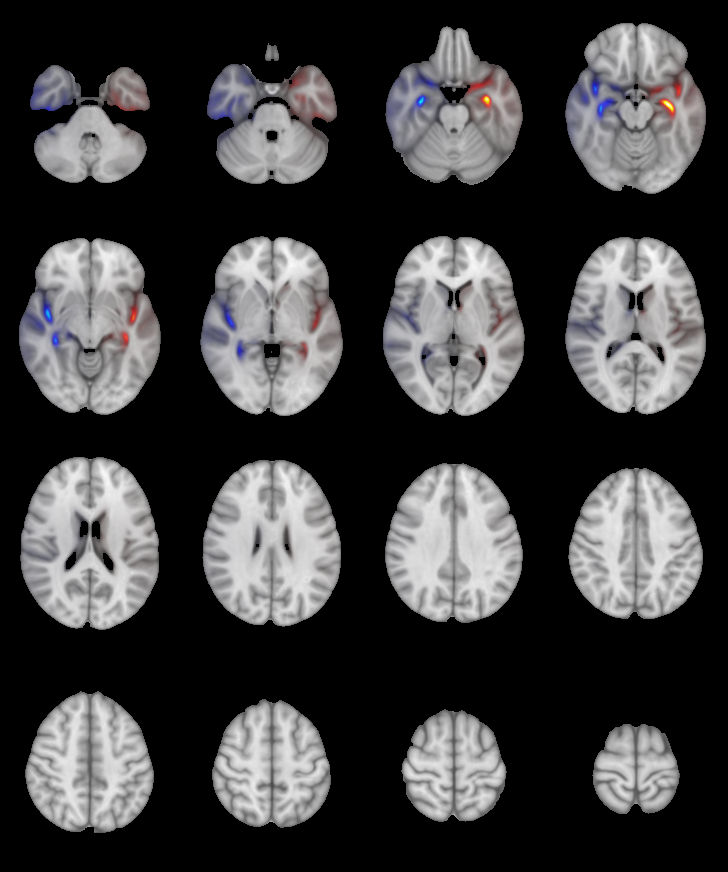
\includegraphics[width=2.5cm]{data/component_1.png}
			};
			\node[] at (5.1, 0) {
				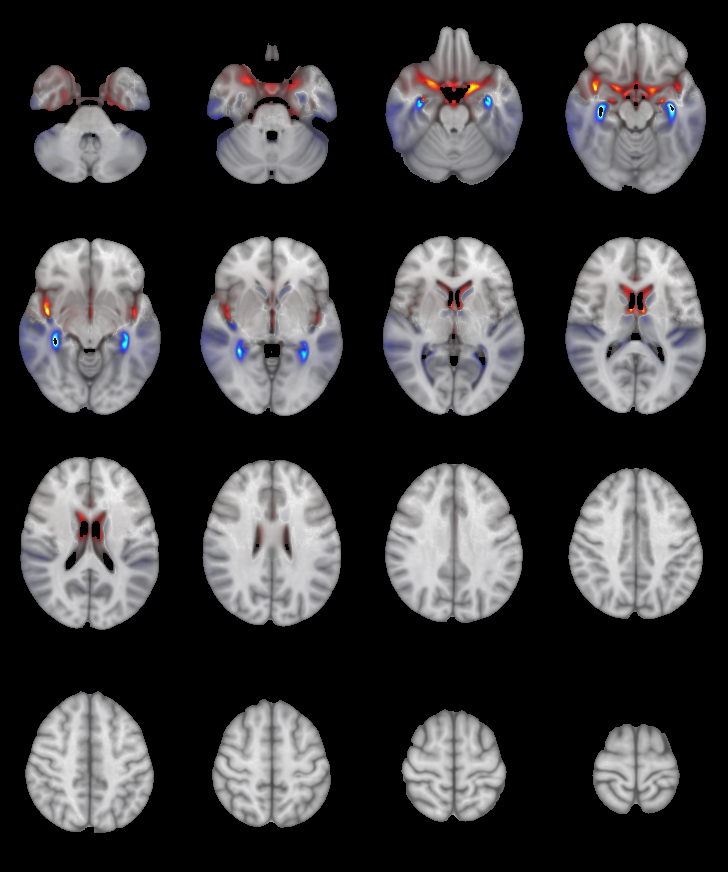
\includegraphics[width=2.5cm]{data/component_2.png}
			};
			\node[] at (7.65, 0) {
				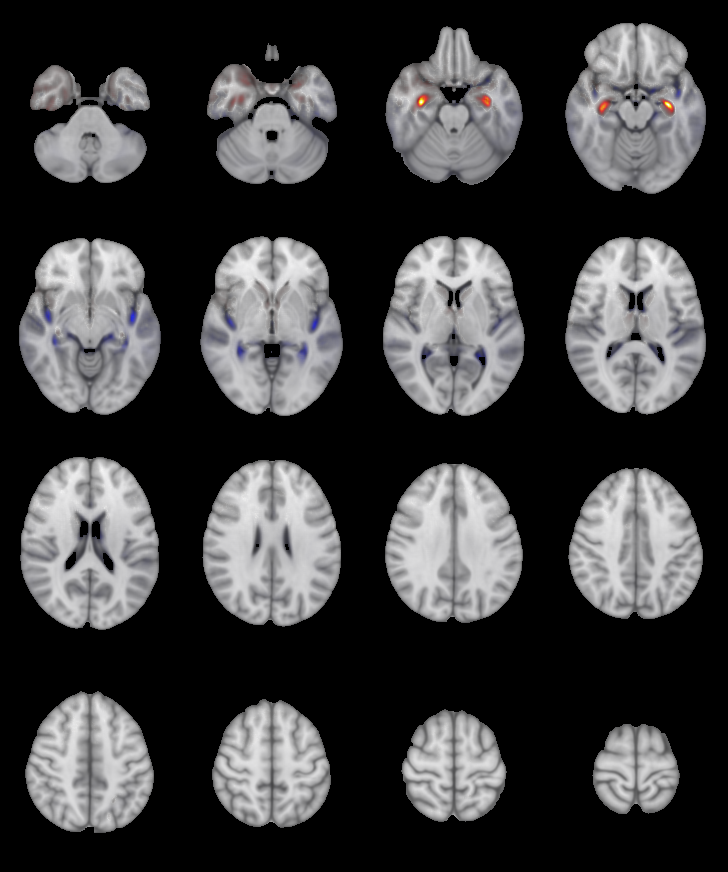
\includegraphics[width=2.5cm]{data/component_3.png}
			};
			\node[] at (0, -4) {};

			\draw[Latex-Latex, very thick] (0, -3.5) -- (7.65, -3.5);
			\draw[very thick] (3.825,-3.575) -- (3.825,-3.425);
			\node[anchor=north] at (3.825,-3.55) {\footnotesize{0}};
			\node[anchor=west] at (7.65,-3.5) {\footnotesize{\textbf{+}}};
			\node[anchor=east] at (0,-3.5) {\footnotesize{\textbf{-}}};
			\node[circle,draw=black,fill=controls-default,inner sep=2pt] (pos) at (6.5,-3.5) {};
			\node[anchor=south] at (pos.north) {
				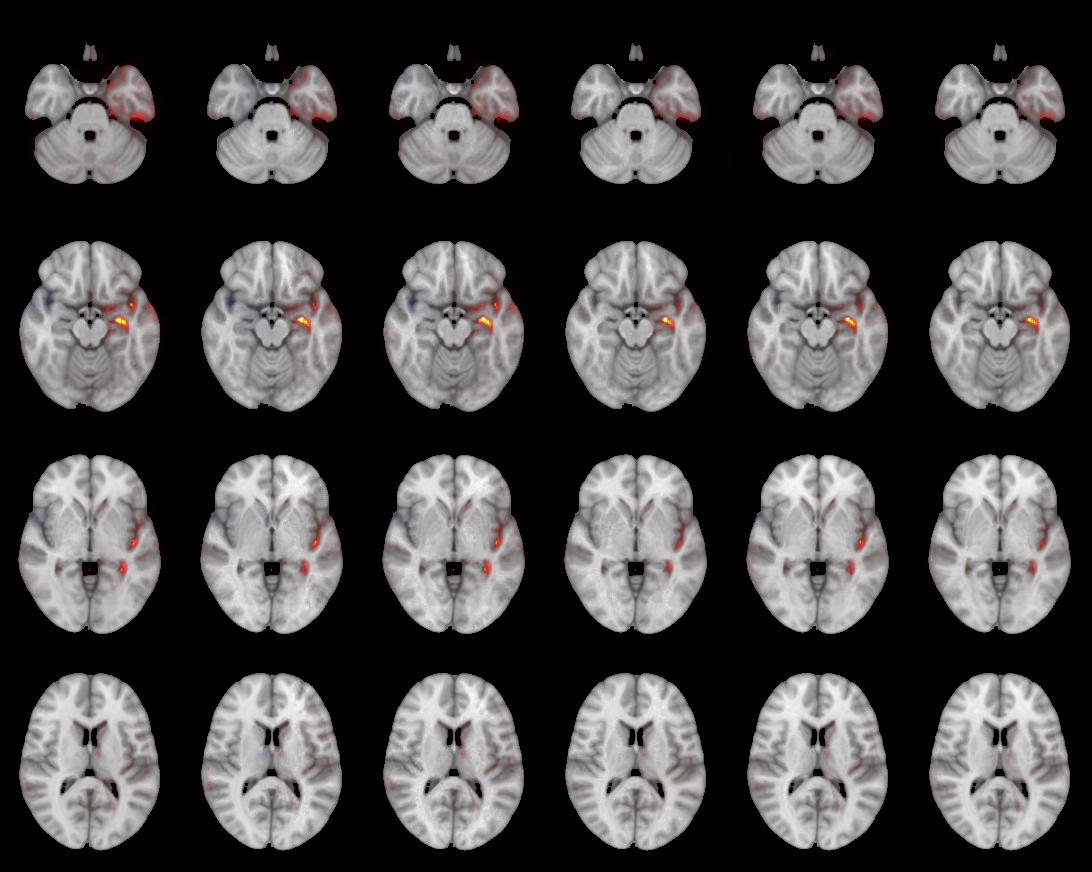
\includegraphics[
					width=1.2cm,
					clip=true,
					trim = 319mm 150mm 0mm 75mm
				]{data/MCI.png}
			};
			\node[circle,draw=black,fill=controls-default,inner sep=2pt] (neg) at (1.15,-3.5) {};
			\node[anchor=south] at (neg.north) {
				\scalebox{-1}[1]{
					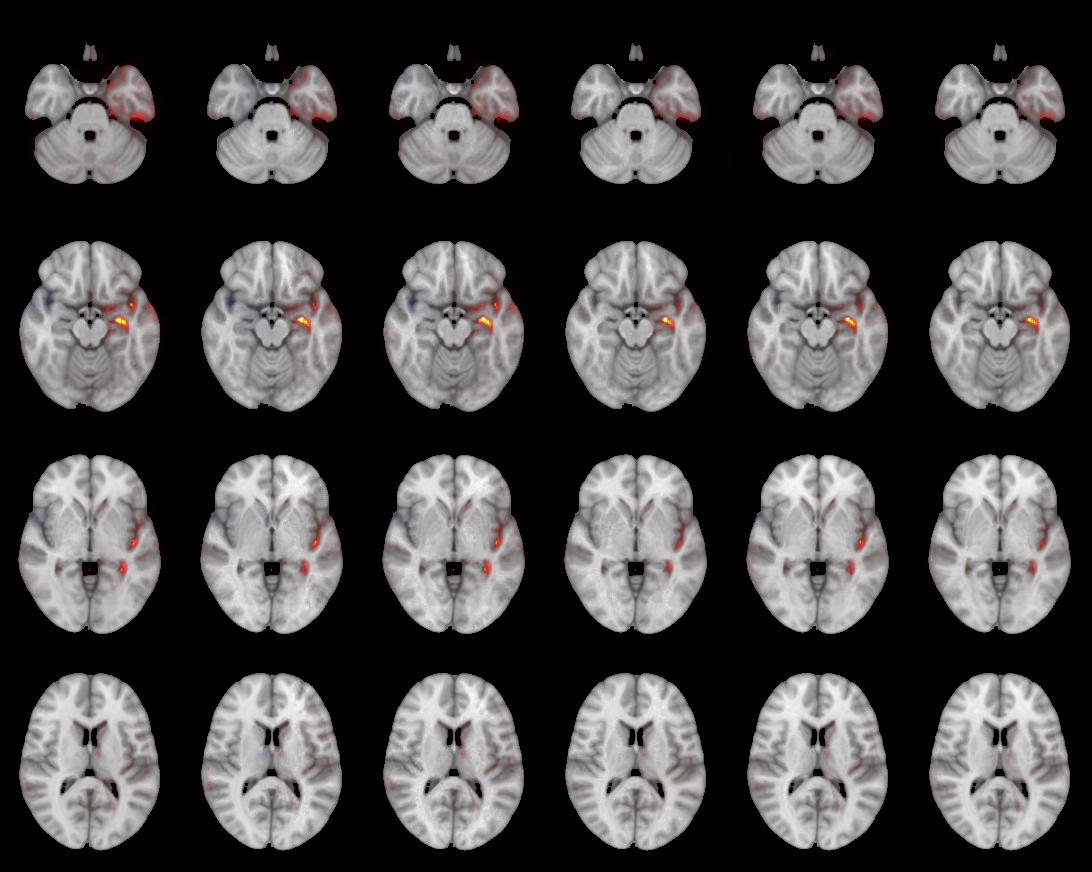
\includegraphics[
						width=1.2cm,
						clip=true,
						trim = 319mm 150mm 0mm 75mm
					]{data/MCI.png}
				}
			};
		\end{tikzpicture}
		\vfill
	\end{frame}

	\begin{frame}{Relevance maps in MCI patients}
		\vfill
		\centering
		\begin{tikzpicture}
			\definecolor{controls-default}{HTML}{3594d6}

			\node[] at (0, 0) {
				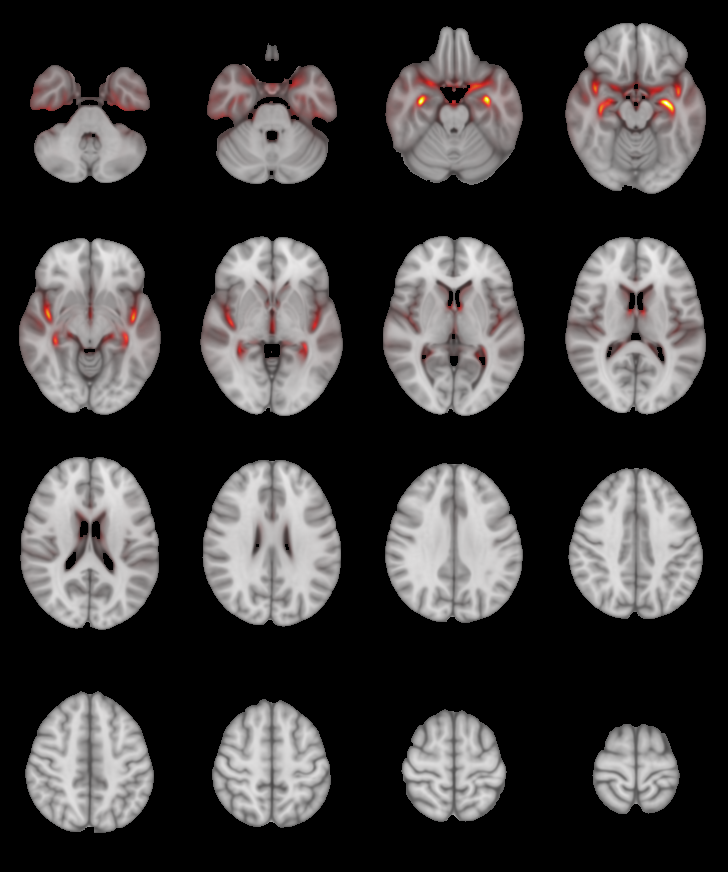
\includegraphics[width=2.5cm]{data/component_0.png}
			};
			\node[] at (2.55, 0) {
				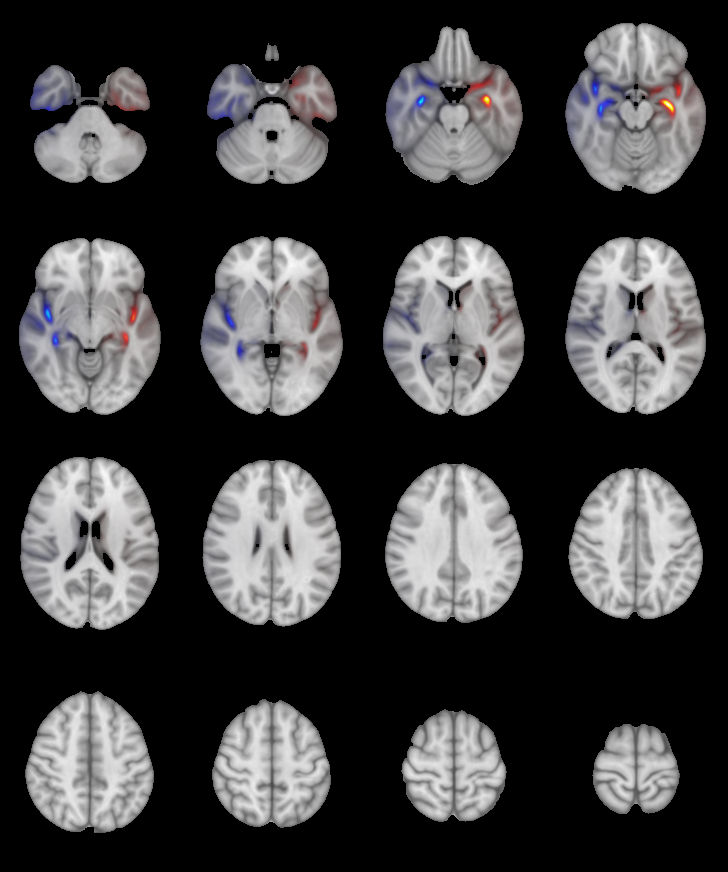
\includegraphics[width=2.5cm]{data/component_1.png}
			};
			\node[] at (5.1, 0) {
				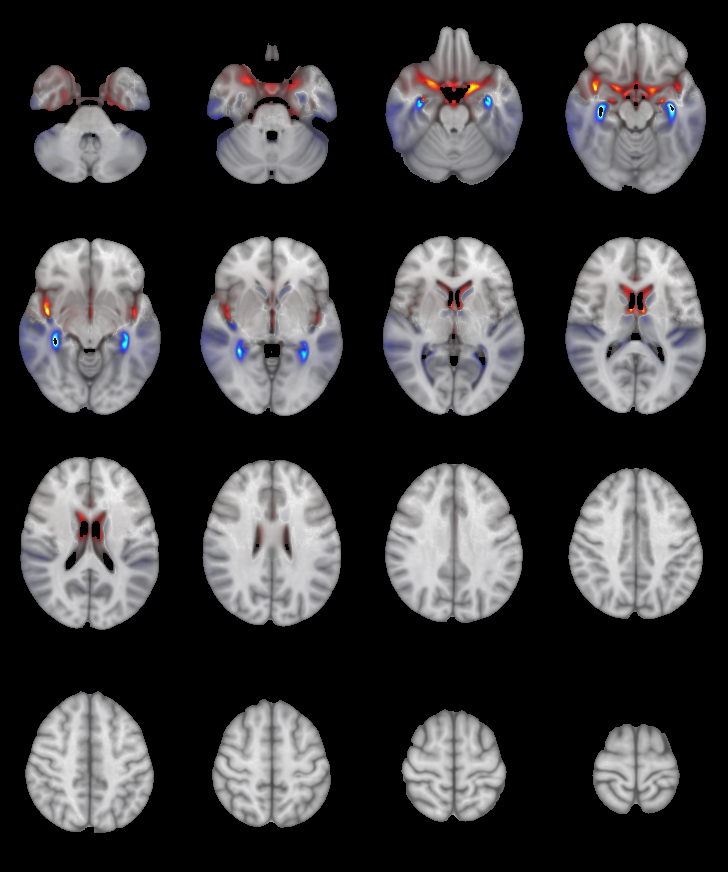
\includegraphics[width=2.5cm]{data/component_2.png}
			};
			\node[] at (7.65, 0) {
				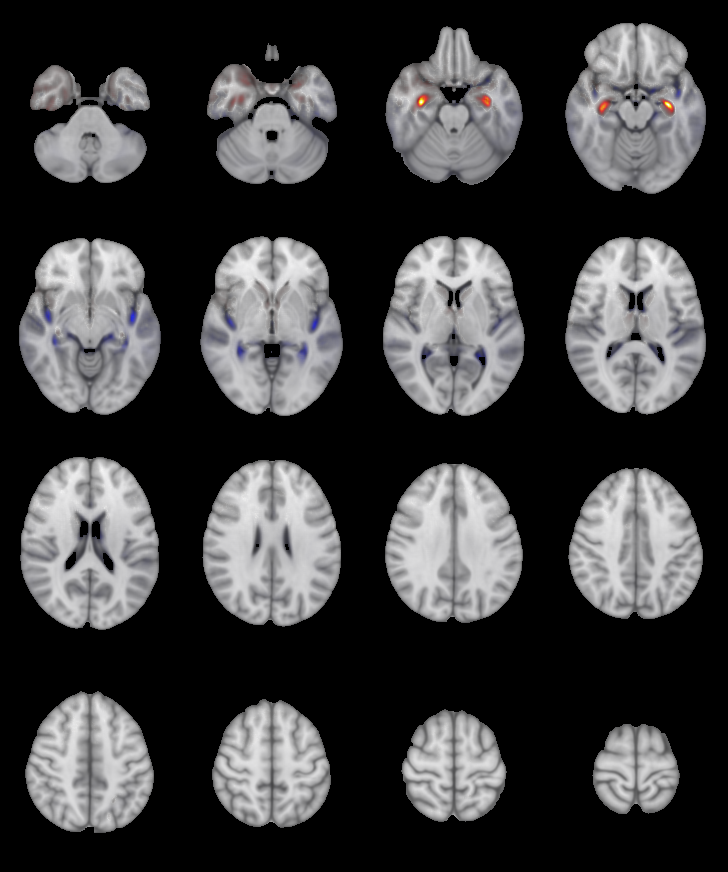
\includegraphics[width=2.5cm]{data/component_3.png}
			};
			\node[] at (0, -4) {};
			\node[] at (0, -1.9) {\scriptsize{$p\mathrm{=}1.19*10^{-15}$}};
			\node[] at (5.1, -1.9) {\scriptsize{$p\mathrm{=}6.62*10^{-4}$}};
			\node[] at (7.65, -1.9) {\scriptsize{$p\mathrm{=}1.06*10^{-5}$}};
		\end{tikzpicture}
		\vfill
	\end{frame}
	\begin{frame}{Summary}
		\vfill
		\centering
		\begin{itemize}
			\item A pipeline for describing individual-level deviations in brain morphology related to dementia using deep learning and explainable AI
			\begin{itemize}
				\item Corroborates existing knowledge
				\item Is predictive of future outcomes
			\end{itemize}
			\item Use cases?
			\begin{itemize}
				\item Fully data-driven characterization of the brain which can be used for e.g. subtyping
				\item Clinical tool?
			\end{itemize}
		\end{itemize}
		\vfill
	\end{frame}
\end{document}
